% 2_literature-review.tex

\cleardoublepage
\chapter{Literature review}\label{chapter:literature-review}
  \textcolor{red}{XXX need to format vehicle tables, like I have for the JAXA TSTO}

	
  \textcolor{red}{
  The study of airbreathing access-to-space systems has been undertaken in some form since the early days of space flight. The prospect of the efficient, cost effective, and reusable space access that airbreathing launch may provide is enticing, and many man-hours and billions of dollars has been expended researching airbreathing launch vehicles. However, airbreathing launch is yet to be realised, due to the large scientific and engineering challenges involved in sending an object to space using airbreathing propulsion. Research is ongoing across many fields and disciplines to develop the designs of airbreathing launch vehicles, including the designs of subsystems such as engines, thermal protection systems, and control systems that can cope with the unique requirements of sustained hypersonic flight. 
}
\textcolor{red}{
  The design of an airbreathing launch system must be determined with careful consideration of the trajectory that the launch system flies to orbit, because the trajectory of a launch system determines the structural and heating loads that are experienced, as well as the necessary control strategy that must be employed to achieve orbit. Accurate trajectory models are required to determine the performance metrics of the launch system, and these initial flight paths are used to guide the design of the launch system.
}



\textcolor{red}{
This section covers the literature available in the areas that are key to developing and analysing the trajectory for a rocket-scramjet-rocket launch system. 
Firstly, a study is conducted on the airbreathing launch systems that have previously been designed and analysed, along with an analysis of the trajectories of these launch systems that may offer valuable insights into the operations of rocket-scramjet-rocket launch systems. Of particular interest are the trajectories of multi-stage airbreathing launch systems, that give insights into the trajectory features that arise from effects of stage separations. 
After this, an overview is given of the optimal control methods that may be used to develop efficient trajectories, along with their applicability to launch vehicle trajectories. 
Lastly, a study is presented on the methods of aerodynamic modelling that may be used to develop dynamic models of the launch system, along with a focussed discussion on the Cart3D program, that is used in this work. 
}

  
  
  \nomenclature[a]{REST}{Rectangular-to-Elliptical Shape Transition}
  
  

   
   
   






    \textcolor{red}{
  \section{Hypersonic Airbreathing Launch Systems and Trajectories}\label{sec:AscentTrajectories}
}
  
%\textcolor{red}{XXX from reviewer: "Significantly expanding Section 2.4 include a more thorough review of air-breathing access to space systems with a particular focus on underlying technologies and their respective strengths and limitations." "Expanding Section 2.5 and 2.6 (on launchers and trajectories) with a focus on critically reviewing the range of methodologies/ constraints/ key assumptions adopted by various authors in developing trajectories for single and multiple-stage to orbit systems. Specific emphasis should be placed on highlighting the shortcomings, methodologies, cost functions, and constraints used in these approaches and how the present work seeks to address them."}
    
Airbreathing access-to-space systems have been investigated in various forms including single-stage, two-stage, and three-stage designs. 
Of these design forms, single-stage and two-stage designs are by far the most common, with very few three-stage designs having been considered to date. This is partly due to the fact that nearly all of the airbreathing launch systems that have been designed are large launchers, designed to launch payloads on the order of thousands of kilograms to orbit. In large launchers, the additional structural mass that results from the addition of engines or subsystems can be mitigated more effectively than for small launcher form factors.
For small satellite launchers, the mass penalties of the systems necessary for airbreathing launch and reusability become more significant, likely necessitating the division of the launcher into separate stages. 
For dedicated small satellite launch, which has become economically feasible only in recent years, a three-stage rocket-scramjet-rocket launcher system has been suggested as a feasible form factor for a small, airbreathing launcher\cite{Preller2017b}. 

 
For any airbreathing launch system, the design of a trajectory during the early design phases is particularly important. Airbreathing launch systems are typically designed using a combination of rocket and airbreathing engines, that have very different requirements for operation. Rocket engines in general perform well from atmospheric to vacuum conditions, while airbreathing engines require relatively high density air and sustained atmospheric flight for operation, which can cause the structural and thermal limits of the vehicle to come into play\cite{Preller2017b}. Figure \ref{fig:FlightCorridor} shows an example flight corridor for an airbreathing launch vehicle, illustrating the upper limits of dynamic pressure at which the structural limits of the launch vehicle are met, and the lower limit of dynamic pressure at which the airbreathing engines are no longer capable of operation. 
\begin{figure}[ht]
	\centering
	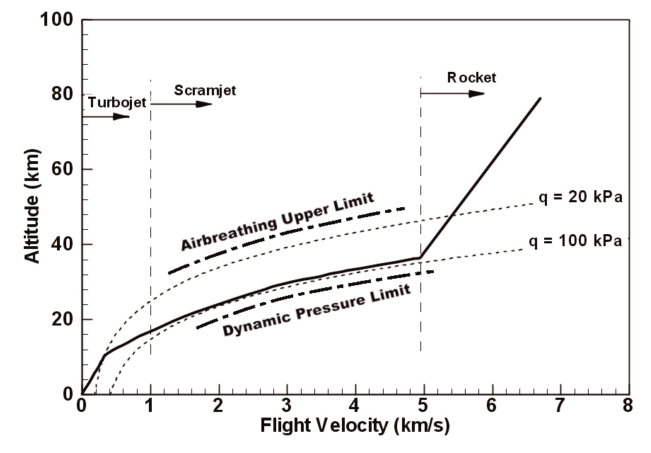
\includegraphics[width=0.7\linewidth]{figures/2_literature-review/FlightCorridor}
	\caption{An example airbreathing flight corridor of an airbreathing launch vehicle\cite{Smart2007a}.}
	\label{fig:FlightCorridor}
\end{figure}
This brings unique complications, as sustained flight in-atmosphere requires a high lift coefficient and results in high structural and thermal loading over long periods, that must be considered during trajectory analysis. In addition, there are a number of design factors that must be considered during trajectory design including;
\begin{itemize}
	\item the requirement for the airbreathing stages to fly in-atmosphere;
	\item the variable efficiency of the airbreathing engines;
	\item the relative efficiency of the different types of engines within the system;
	\item the aerodynamic performance of each vehicle or engine-mode of the system;
	\item and the structural limitations of the system.
\end{itemize}
These factors cause trade-offs between the stages of the launch system\cite{Staufenbiel2000}, and limit the operational regime of the launch system.


As well as complex trade-offs during ascent, the reduced fuel usage of airbreathing engines changes the mass distribution of airbreathing launch systems and generally have a high lift-to-drag ratio that allows for the fly-back and landing of some or all of the launch system in a similar manner to a conventional aircraft\cite{Preller2017b}. The return portion of the trajectory must be considered in the trajectory analysis and concurrent design for reusable launch systems, in order to develop a launch system design that is capable of being reused efficiently\cite{Hellman}. This brings additional considerations to the vehicle and trajectory design, because the vehicle must be designed to withstand the conditions of return as well as launch, and must be physically able to return and land at a suitable location\cite{Hellman}. The trajectory analysis of a reusable vehicle is particularly important, because the viability of returning the vehicle to a suitable landing location must be determined, and the impact of the return trajectory on the launch flight profile must be established. The fly-back can be a high-impact design driver, with the performance of the vehicle relying significantly on an efficient return flight\cite{Tetlow1992,Hellman}. 

This study aims to understand the optimal trajectory of a rocket-scramjet-rocket multi-stage launch system, that may be considerably different to other configurations of airbreathing launchers. 
To this end, this section investigates the designs of all forms of airbreathing launch systems that have been developed, along with their trajectories. The manner in which the design and number of stages of the launch systems influences their trajectories is studied, allowing for some key features of airbreathing launch system trajectories to be identified.
  
 
  
  
  
  
  
  
 
  
  
 \textcolor{red}{
  \subsection{Single Stage Airbreathing Launch Systems}
}

\afterpage{
	\begin{landscape}% Landscape page
%\begin{table}[ht]
\begin{xltabular}{\linewidth}{|X|X|X|}
\hline \small  \textbf{Launcher} &\small \textbf{Design} &\small \textbf{Trajectory}\\ 
\hline \small \textbf{X-30} (NASP)\cite{NASP} \newline \newline Conceived as a technology demonstrator for the NASP program, the X-30 would have been the first airbreathing launch system to be operationally demonstrated, but its program was cancelled prematurely. Many important aspects of the X-30 have not been made public\cite{NASP} and so details on this vehicle are incomplete.   
&\small
\raisebox{-\totalheight}{\includegraphics[width=0.5\linewidth]{"figures/2_literature-review/X30"}} 

$\cdot$\textbf{Mass:} Designs studied with a range of 'less than 200000lbs and greater than 300000lbs'\cite{NASP} (90718.5 - 136077.7kg).

$\cdot$\textbf{Propulsion:} Powered by scramjets with reusable rocket engines or RBCC engines.

&\small
\raisebox{-\totalheight}{\includegraphics[width=0.5\linewidth]{"figures/2_literature-review/X30Traj"}} 

$\cdot$\textbf{Launch:} Horizontal.
\\
\hline\small \textbf{Langley Accelerator} (NASP)\cite{WCC,Powell1991,Lu1993} 
\newline  \newline Developed as a standardised vehicle for single-stage-to-orbit airbreathing launcher studies, the Langley Accelerator was not intended to be an operational concept. The version developed by Powell et al.\cite{Powell1991} is presented here. 
&
\small
\raisebox{-\totalheight}{\includegraphics[width=0.5\linewidth]{"figures/2_literature-review/Powell Vehicle"}} 

$\cdot$\textbf{Mass:} 136079kg.

$\cdot$\textbf{Length:}  61m.

$\cdot$\textbf{Propulsion:} Fully airbreathing in-atmosphere, rockets for circularisation.

&
\small
\raisebox{-\totalheight}{\includegraphics[width=0.5\linewidth]{"figures/2_literature-review/Powell Trajectory"}} 

$\cdot$\textbf{Launch:} Horizontal. 

$\cdot$\textbf{Trajectory:} Maximum dynamic pressure reached as rapidly as possible, and flown until pull-up is performed under the power of the scramjet engines. 

$\cdot$\textbf{Return:} Coast phase after scramjet shutdown until circularisation by rocket engines.

 \\ 
 \hline \small \textbf{HOTOL}\cite{Aberleen}\newline\newline
 The British HOTOL concept was a single-stage-to-orbit spaceplane developed initially as a proof-of-concept study in 1982, but later courted to the ESA as a major project and refused. Funding was withdrawn in 1982 before development could commence. 
 & \small
 \raisebox{-\totalheight}{\includegraphics[width=0.5\linewidth]{"figures/2_literature-review/HOTOL"}}
 $\cdot$\textbf{Payload:} 7-10t.
 
 $\cdot$\textbf{Length} 62m.
 
 $\cdot$\textbf{Propulsion:} Four Swallow engines, operating in airbreathing mode until 26km altitude, and rocket mode thereafter.
 & \small
 $\cdot$\textbf{Trajetory:} No detailed trajectory information is readily available. 
 \\
\hline \small\textbf{ABLV-GT} (Hyper-X)\cite{Bradford2000, HyperX} 
\newline \newline 
The ABLV-GT was developed by Georgia Tech Space Systems Design Lab as an extension of the ABLV (airbreathing launch vehicle) design study performed by NASA, aiming to develop a conceptual design for a realistic launch vehicle. This vehicle has strong links to the Next Generation Launch Technology Program, a successor to the NASP program, which produced the X-43 test vehicle, the first demonstrator of scramjet operation in free-flight.
&
\small
\raisebox{-\totalheight}{\includegraphics[width=0.5\linewidth]{"figures/2_literature-review/HyperX"}}

$\cdot$\textbf{Note:} X-43A shown as a representative vehicle shape.

$\cdot$\textbf{Mass:} 13520000lbs

$\cdot$\textbf{Length:} 190.5ft.

$\cdot$\textbf{Propulsion:} Powered by turboramjet \& RBCC engines.

&
\small
\raisebox{-\totalheight}{\includegraphics[width=0.5\linewidth]{"figures/2_literature-review/ABLV-GTTraj"}}

$\cdot$\textbf{Launch:} Horizontal. 

$\cdot$\textbf{Trajectory:} Maximum dynamic pressure flight during majority of ram/scramjet operation followed by a pull-up upder rocket-augmented scramjet power. 
\\ 
\hline\small \textbf{GTX} (Trailblazer)\cite{Roche2000,Trefny1999} 
\newline \newline 
The GTX (formerly Trailblazer) was another offshoot of the ABLV program.
&
\small \raisebox{-\totalheight}{\includegraphics[width=0.5\linewidth]{"figures/2_literature-review/GTX"}} 

$\cdot$\textbf{Payload:} 25000lbs.

$\cdot$\textbf{Mass:} 1252617lbs.

$\cdot$\textbf{Length:} 263.5ft.


$\cdot$\textbf{Propulsion:} Ramjet-scramjet-rocket propulsion. 
 
&
\small \raisebox{-\totalheight}{\includegraphics[width=0.5\linewidth]{"figures/2_literature-review/GTXTraj"}}

$\cdot$\textbf{Launch:} Vertical. 

$\cdot$\textbf{Trajectory:} Flight at maximum dynamic pressure of 2000psfa (95.76kPa) followed by a pull-up under scramjet power, when the maximum Mach limit of the scramjet is reached. Rocket power is used to accelerate to orbit. 
 \\
\hline \small\textbf{Lazarus}\cite{Young2006} \newline \newline 
The Lazarus concept was developed at the Georgia Institute of Technology Space Systems Design Lab, as an SSTO concept for medium size payload launch, with a secondary purpose of use as a global strike platform. 

&\small \raisebox{-\totalheight}{\includegraphics[width=0.5\linewidth]{"figures/2_literature-review/Lazarus"}}  

$\cdot$\textbf{Payload:} 5000lbs (2268.0kg)..

$\cdot$\textbf{Mass:} 180000lbs (81646.6kg).

$\cdot$\textbf{Length:} 102.8ft (31.3m). 


$\cdot$\textbf{Propulsion:} RBCC engines with high energy density material fuel. A sled is used for takeoff, that provides fuel to the RBCC engines. 

&\small \raisebox{-\totalheight}{\includegraphics[width=0.5\linewidth]{"figures/2_literature-review/LazarusTraj"}}

$\cdot$\textbf{Launch:} Horizontal using sled.

$\cdot$\textbf{Trajectory:} Maximum dynamic pressure flight during airbreathing operation at 1800psf (86.2kPa). At Mach 10 a pull-up is initiated using combined scramjet-rocket propulsion. At the minimum operable conditions of the scramjet engines, the rocket takes over to accelerate to orbit. 

$\cdot$\textbf{Return:} Return trajectory is not considered. \\

\hline \small\textbf{Hyperion}\cite{Hyperion}\newline \newline 
The Hyperion was developed by Georgia Tech Space Systems Design Lab, as an assessment of the 'Vision Vehicle' design class, solicited by NASA as part of the Advanced Reusable Technologies Program. Hyperion was conceptualised to assess whether RBCC propulsion and other advanced technologies can significantly reduce the cost of space access. 
&\small \raisebox{-\totalheight}{\includegraphics[width=0.5\linewidth]{"figures/2_literature-review/Hyperion"}}  

$\cdot$\textbf{Payload:} 20000lbs (9071.8kg) to LEO. 

$\cdot$\textbf{Mass:} 800700lbs (363191.4kg).

$\cdot$\textbf{Length:} 179ft (54.6m). 



$\cdot$\textbf{Propulsion:} Powered by 5 RBCC engines, with return flight suplemented by low-thrust H2 ducted fans. 

&\small \raisebox{-\totalheight}{\includegraphics[width=0.5\linewidth]{"figures/2_literature-review/HyperionTraj"}} 

$\cdot$\textbf{Launch:} Horizontal.

$\cdot$\textbf{Trajectory:} Flight at maximum dynamic pressure of 2000psf (95.76kPa) during airbreathing operation. Pull-up during scramjet operation, with transition to rocket mode during pull-up. 

$\cdot$\textbf{Return:} No Return trajectory considered.

\\
\hline \small\textbf{Argus}\cite{Argus} \newline\newline
The Hyperion was developed by Georgia Tech Space Systems Design Lab, in support of NASA's Highly Reusable Space Transportation study. The Argus was a conceptual design intended to be investigated and compared to other classes of launchers to determine cost effective long term solutions to space access.  
&\small
\raisebox{-\totalheight}{\includegraphics[width=0.5\linewidth]{"figures/2_literature-review/Argus"}}

$\cdot$\textbf{Payload:} 20000lbs (9071.8kg).

$\cdot$\textbf{Mass:} 597250lbs (270908.0kg).

$\cdot$\textbf{Length:} 171ft (52.1m). 

$\cdot$\textbf{Propulsion:} Initially accelerated along a maglifter track. Afterwards powered by two RBCC ejector-ramjet engines, with OMS thrusters used for circularisation and manoeuvring on-orbit. 

&\small
$\cdot$\textbf{Launch:} Horizontal on maglifter track. 

$\cdot$\textbf{Trajectory:} After launch, accelerated using ejector ramjet so that maximum dynamic pressure of 1500psf (71.8kPa) is reached at transition to fan-ramjet mode. 
At Mach 6, transition to rocket mode occurs for acceleration to parking orbit.\\ 

\hline 
\end{xltabular} 
		%\end{table}
	\end{landscape}
}

A single stage launch system design aims to achieve space launch with only one vehicle, and generally no separation of mass until payload deployment. Table XXX summarises the recent single-stage-to-orbit airbreathing launchers that have been developed as detailed designs, along with their key design and trajectory features. 

All of the single stage-to-orbit (SSTO) airbreathing launch vehicles that have been studied are designed to be fully reusable. Being fully reusable is the primary attraction of the SSTO spaceplane, and indeed is likely to be the only way in which a system of this type is able to be financially viable. 
The single-stage form factor is in general convenient for reusability, as the additional structural and subsystem complexity necessary to facilitate return is mitigated by having only one large vehicle. SSTO vehicles also have the advantage of not needing to stage, saving on the additional system weight and complexity required when staging in atmosphere. 
However, SSTO launch vehicles are required to accelerate the entire launch system to orbital or near-orbital speeds, and exit the atmosphere completely. This introduces significant complexity to the return flight and reuse of SSTO systems, which are required to re-enter the atmosphere at orbital speeds\cite{NASP}. This reentry poses significant challenges to the thermal and structural protection and control subsystems of SSTO vehicles, particularly when a primary design driver is cost efficiency.
 Accelerating an entire launch system to orbit also results in a significant amount of 'dead-weight', ie. subsystems that are designed for use only in a specific part of a launch, that must nonetheless be transported to orbit and back. In particular for airbreathing SSTO systems, this 'dead-weight' derives from the need to carry multiple engines that are switched between during flight. This means that airbreathing SSTO launch systems are generally highly fuel efficient at all stages of flight, but carry heavy engines that are not used in all flight regimes. 
To mitigate this 'dead-weight', SSTO vehicles are generally powered by rocket-based combined cycle (RBCC) engines which are capable of operating in various airbreathing or air-assisted rocket modes using common engine components, sometimes augmented by turbojet engines for efficient power during launch or return flight. Despite this mitigation measure, the many subsystems required by SSTO launch systems are complex and heavy, and are likely to also be extremely costly.
For this reason, all of the SSTO airbreathing launchers that have been investigated are designed for medium-to-large payload launch, and are large, heavy vehicles, with design profiles incorporating many aircraft-like features such as wings, tails and aerodynamic control surfaces. 

The ascent trajectories of SSTO airbreathing launch vehicles are significantly different from all-rocket launch systems, due to their airbeathing engines requiring atmosphere to operate, necessitating the launch vehicle spending a large amount of time flying close to horizontal.
Most SSTO airbreathing systems are designed to be horizontally launched, under turbojet or rocket-assisted power. The exception to this is the GTX, which launches vertically under rocket power\cite{Roche2000,Trefny1999} . 
All of the SSTO vehicles examined follow a constant dynamic pressure trajectory during the majority of airbreathing hypersonic flight, at a low trajectory angle, to allow the efficient operation of their airbreathing engines. 
Constant dynamic pressure flight advantageous for an airbreathing accelerator due to the trade-off between structural loading and engine performance\cite{Olds1998}. As dynamic pressure increases so does the structural loading on the vehicle, however the performance of a ramjet or scramjet engine is directly reliant on dynamic pressure\cite{Olds1998}. A constant dynamic pressure trajectory is viewed as being an acceptable compromise between these two factors when designing a launch vehicle, operating at the dynamic pressure limit of the launch vehicle. 
Although a constant dynamic pressure trajectory is likely to produce high efficiency flight for the high speed airbreathing portion of an ascent trajectory, there are a variety of factors that must be considered in designing the trajectory of a launch system. 
For example, a constant dynamic pressure flight may produce suboptimal conditions for the switch from airbreathing engines to rocket power for exoatmospheric flight. For this reason, most of the vehicles studied then perform a pull-up manoeuvre during airbreathing operation, before or during the transition to rocket-power. 
At the end of airbreathing operation it is often more optimal for the vehicle to fly at less than maximum dynamic pressure for a time during airbreathing engine operation, allowing the trajectory angle and altitude to be raised before the rocket engines are powered-on. 
This trajectory shape trades off the performance of the airbreathing engines for altitude before the rocket engines are powered on fully, and has been shown to be the optimal trajectory throughout the studies of the vehicles covered in Table XXX\cite{Argus,Powell1991,Trefny1999,Roche2000,Pescetelli2012,Young2006,Bradford2000,Hyperion}, as well as for generic trajectory optimisation studies that do not develop a detailed vehicle design\cite{Pescetelli2012,Mooij,Lu1993}.
A pull-up was found to be optimal for vehicles where the rocket engines are not ignited until circularization altitude\cite{Powell1991,Lu1993}, vehicles where the rocket engine is ignited immediately after airbreathing engine cut-off\cite{Trefny1999,Roche2000,Pescetelli2012} as well as for vehicles that operate in combined scramjet-rocket mode\cite{Young2006,Bradford2000}.
For SSTO vehicles a pull-up manoeuvre is a trade-off between the altitude at airbreathing engine cut-off and the velocity achievable at cut-off. Due to the entire vehicle being lifted into orbit, this generally becomes a relatively simple problem of engine efficiency. The airbreathing engine is used for its high efficiency, until the dynamic pressure drops below the operable limit of the airbreathing engine, or until the thrust provided by the airbreathing engine is significantly counteracted by the effects of drag and gravity. 

While the SSTO launch systems and trajectory shapes that have been studied have indicated that horizontal flight at close to maximum dynamic pressure, with a period of flight at off-maximum dynamic pressure at some points during the trajectory to trade-off efficiency between flight modes, these analyses of SSTO vehicles can only be indirectly applied to multi-stage vehicles. SSTO vehicles must necessarily carry their whole mass to orbit, due to a lack of stage transitions, and as such may not behave in the same manner as multi-stage vehicles, and may be designed considerably differently. For this reason, the designs and trajectories of multi-stage airbreathing launch systems must be primarily used to inform decisions on the design and optimal flight paths of new multi-stage designs. 
  	
  \textcolor{red}{
  \subsection{Two-Stage Launch Systems} \label{sec:twostagelaunchers}
}

% For claim of first detailed examination of the optimal trajectory of a multi-stage vehicle, see comments in each table. 


\afterpage{
\begin{landscape}
\begin{xltabular}{\linewidth}{|X|X|X|}
	\hline \small  \textbf{Launcher} &\small \textbf{Design} &\small \textbf{Trajectory}\\ 
	\hline \small 
	\textbf{LaRC Turboramjet}\cite{Wilhite1991}\newline\newline
	The LaRC boosters were developed by Wilhite et al.\cite{Wilhite1991} in order to test the effects of staging Mach number on a two-stage system. These boosters were studied as part of the NASP program, and were intended only to be used as a representative vehicle for research purposes.  

	&\small
	\raisebox{-\totalheight}{\includegraphics[width=\linewidth]{"figures/2_literature-review/WilHite Booster Vehicle"}}
	
	$\cdot$\textbf{Reusability:} Fully reusable.
	
	$\cdot$\textbf{Mass:} Nominal gross takeoff weight of approximately 360klb (160Mg), although this varies with staging Mach number. 
	
	$\cdot$\textbf{Payload:} 10000lbs (4535.9kg) to LEO. 
	
	$\cdot$\textbf{Propulsion:} First stage propulsion is rocket-turboramjet, second stage propulsion is rocket. 
	
	
	&\small
	\raisebox{-\totalheight}{\includegraphics[width=\linewidth]{"figures/2_literature-review/WilHite Booster Trajectory"}}
	
	$\cdot$\textbf{Launch:} Horizontal.
	
	$\cdot$\textbf{Airbreathing Trajectory:} Constrained to maximum dynamic pressure of 1000psf (47.9kPa) until the staging Mach number of 5,6 or 7 is reached. A pull-up occurs at nominal staging Mach number under ramjet power, to reach the prescribed staging dynamic pressure of 300psf (14.4kPa). Pull-up occurs at a 2g constrained rate. 
	
	$\cdot$\textbf{Orbiter Trajectory:} Undefined.
	
	$\cdot$\textbf{Return Trajectory:} Unpowered turn and deceleration, followed by a turbojet powered cruiseback. 
	\\
	
	
	\hline \small 
	\textbf{JAXA TSTO Spaceplane}\cite{Fujikawa2017}\newline\newline
	Fujikawa et al.\cite{Fujikawa2017} have developed a spaceplane as a feasibility study on TSTO fully-reusable launch for JAXA. 
	
	% (NOTE: 2DOF no return)? end text of p 272 in interesting}
	&\small
	\raisebox{-\totalheight}{\includegraphics[width=\linewidth]{"figures/2_literature-review/Tsuchiya Vehicles"}}
	
	$\cdot$\textbf{Reusability:} Fully-reusable. 
	
	$\cdot$\textbf{Propulsion:} First stage RBCC, second stage rocket. 
	
	$\cdot$\textbf{Payload:} 800kg.

	 $\cdot$\textbf{Mass:} Booster 533.8t, orbiter 47.1t.
	 
	 $\cdot$\textbf{Length:} Booster 38.4m, orbiter 18.8m. 
	 
	
	&\small
	\raisebox{-\totalheight}{\includegraphics[width=\linewidth]{"figures/2_literature-review/Tsuchiya"}}
	
	$\cdot$\textbf{Launch:} Horizontal. 
	
	$\cdot$\textbf{Airbreathing Trajectory:} Majority of flight is at less than maximum dynamic pressure in order to improve the performance of the RBCC engines due to external nozzle effects. A pull-up is performed during scramjet operation, explained as part of the RBCC performance improvement.

	
	$\cdot$\textbf{Return Trajectory:} Not simulated. 
	
	\\
	\hline \small 
	\textbf{NASA Ames TSTO Spaceplane}\cite{Mehta2001}\newline\newline
	A TSTO spaceplane was conceptualised by Mehta and Bowles\cite{Mehta2001}, based on a '93 design for the NASP program. This concept was designed to be economically viable launcher, with built-in growth potential. 
	&\small
	\raisebox{-\totalheight}{\includegraphics[width=0.48\linewidth]{"figures/2_literature-review/Mehta Vehicle"}}
	\raisebox{-\totalheight}{\includegraphics[width=0.48\linewidth]{"figures/2_literature-review/Mehta Vehicle2"}}
	
	$\cdot$\textbf{Reusability:} Fully reusable.
	
	$\cdot$\textbf{Payload:} 25000lbs (11339.8kg).
	
	$\cdot$\textbf{Propulsion:} Booster propulsion system is tubojet/ramjet/scramjet while orbiter has standard LOX/H2 rocket propulsion. 
	
	$\cdot$\textbf{Mass:} Booster: 602300lbs (273198kg), Orbiter: 199301lbs (90401kg).
	
	$\cdot$\textbf{Length:} Booster: 224ft (68.3m), Orbiter: 64.5ft (19.7m).
	&\small
	\raisebox{-\totalheight}{\includegraphics[width=\linewidth]{"figures/2_literature-review/Mehta Trajectory"}}
	
	$\cdot$\textbf{Launch:} Horizontal.
	
	$\cdot$\textbf{Airbreathing Trajectory:} Acceleration before the hypersonic regime is achieved steadily, with an increase in altitude at the transonic 'pinch point' to reduce dynamic pressure. 
	During the hypersonic regime, a constant dynamic pressure of 2100lb/ft2 (100.5kPa) until Mach 10.
	At Mach 10, a 2g pull-up is initiated, to lower the dynamic pressure to 300lb/ft2 (14.4kPa) for separation, and to improve the flight path angle at separation. The scramjet engines are cut off at the start of this pull-up.  
	
	$\cdot$\textbf{Orbiter Trajectory:} Ascent under rocket power. 
	
	$\cdot$\textbf{Return Trajectory:} The booster initiates a turn, and cruises back under turbojet power. 
	The orbiter reenters and returns unpowered. 
	
	\\
	\hline \small 
	\textbf{Tohoku University TSTO Launcher}\cite{Takahashi1997}\newline\newline
	Developed by Takahashi et al.\cite{Takahashi1997}, a conceptual TSTO system was designed to investigate acceptable launch, landing and abort sites along the coast of the Japanese islands. 
	&\small
	\raisebox{-\totalheight}{\includegraphics[width=\linewidth]{"figures/2_literature-review/Takahashi Vehicle"}}
	
	$\cdot$\textbf{Reusability:} Partially reusable, first stage only. 
	
	$\cdot$\textbf{Payload:} 2000kg to LEO. 
	
	$\cdot$\textbf{Mass:} Booster: 75.0ton, Orbiter: 19.7ton.
	
	$\cdot$\textbf{Length:} Booster: 30m,  Obiter: 19m.
	
	$\cdot$\textbf{Propulsion:} The booster uses the air-turbo-ramjet engine developed at Japan's Institute for Space and Astronautical Science. The orbiter uses the LE-5B rocket engine. 
	
	
	&\small
	\raisebox{-\totalheight}{\includegraphics[width=\linewidth]{"figures/2_literature-review/Takahashi Trajectory"}}
	
	$\cdot$\textbf{Launch:} Horizontal.
	
	$\cdot$\textbf{Airbreathing Trajectory:} Flight at a maximum dynamic pressure of 50kpa. 
	
	$\cdot$\textbf{Orbiter Trajectory:} Separation at Mach 6 and 50kPa dynamic pressure, followed by a pull-up to orbit under rocket power. 
	
	$\cdot$\textbf{Return Trajectory:} Glide to a landing site downrange.
	
	
	\\
	\hline \small 
	\textbf{S{\"a}nger (Saenger)}\cite{Aberleen}\newline\newline
	The S{\"a}nger was a German TSTO alternative to the HOTOL. S{\"a}nger was intended to drive studies and technology development within the German Hypersonic Technology Program (HTP). 
	
	
	&\small
	\raisebox{-\totalheight}{\includegraphics[width=\linewidth]{"figures/2_literature-review/Saenger"}}
	
	$\cdot$\textbf{Reusability:} First stage reusable. Two alternative upper stages; a reusable, manned version for a crew of four and 3t payload, and an expendable cargo version for carrying 7-8t payload to LEO. 
	
	$\cdot$\textbf{Mass:} Booster: 405t. 
	
	$\cdot$\textbf{Length:} Booster: 82.5m.
	
	$\cdot$\textbf{Propulsion:} First stage powered by tubojets and ramjets, with upper stages powered by conventional LOX/LH2 rockets. 
	
	&\small
	$\cdot$\textbf{Trajectory:} No detailed trajectory information available beyond separation to second stage at Mach 6.6. 
	\\
	\hline \small 
	\textbf{Dassault Aviation Star-H / HERMES} \cite{Aberleen}\newline\newline
Developed by Dassault, the STAR-H was the French study that sought to mirror the HOTOL and S{\"a}nger with the design of an aerospace plane capable of servicing the ISS. The STAR-H incorporates the Hermes, a Euopean manned launcher concept, as 'payload' making it essentially a two-and-a-half stage vehicle. 
	
	%https://books.google.com.au/books?id=vLadDQAAQBAJ&pg=PA178&lpg=PA178&dq=dassault+starh&source=bl&ots=FzPe3XdDWu&sig=ACfU3U3dDHG34_X23TOZZcmJMjKLW-eMGw&hl=en&sa=X&ved=2ahUKEwiphJi588zjAhVFfX0KHTuGBCsQ6AEwB3oECAgQAQ#v=onepage&q=dassault%20starh&f=false
	
	%https://books.google.com.au/books?id=06UzDwAAQBAJ&pg=PA173&lpg=PA173&dq=starh+launcher&source=bl&ots=bo5UbMwTGU&sig=ACfU3U1V86V5Gkzmpd74tfExJkxzv6ugow&hl=en&sa=X&ved=2ahUKEwjqj6es88zjAhXUXCsKHTitCnwQ6AEwCnoECAgQAQ#v=onepage&q=starh%20launcher&f=false
	&\small
\raisebox{-\totalheight}{\includegraphics[width=\linewidth]{"figures/2_literature-review/StarH"}}

$\cdot$\textbf{Reusability:} Reusable first stage, expendable orbiter, 'payload' of a small spaceplane glider is also reusable. 

$\cdot$\textbf{Mass:} Booster 299t, orbiter 101t. 

$\cdot$\textbf{Propulsion:} First stage powered by five combined cycle engines, second stage rocket powered. 
	
	&\small
	$\cdot$\textbf{Airbreathing Trajectory:} No detailed trajectory information is available beyond separation to second stage at Mach 6. 
	
	\\
	\hline \small 
	\textbf{Starsaber}\cite{Germain2001}\newline\newline
	Starsaber was a conceptual design produced by the Georgia Institute of Technology Space Systems Design Lab, with the collaboration of NASA's Marshall Space Flight Centre. Starsaber was intended to investigate the feasibility of RBCC engines for small payload class missions. 
	&\small
	\raisebox{-\totalheight}{\includegraphics[width=\linewidth]{"figures/2_literature-review/Starsaber"}}
	
	$\cdot$\textbf{Reusability:} Partially reusable. First stage reusable, second stage expendable. 
	
	$\cdot$\textbf{Payload:} 300lbs (136kg). 
	
	$\cdot$\textbf{Mass:} Booster: 79150lbs (35902kg), Orbiter: 3400lbs (1542kg). 
	
	$\cdot$\textbf{Length:} Booster: 77ft (23.5m), Orbiter 13.1ft (4.0m).
	
	$\cdot$\textbf{Propulsion:} The booster is powered by two RBCC (ejector-ramjet/ramjet/rocket) engines, while the orbiter is powered by rocket engines.  
	
	&\small
	\raisebox{-\totalheight}{\includegraphics[width=\linewidth]{"figures/2_literature-review/StarsaberTraj"}}
	
	%$\cdot$Trajectory optimised in separate stages for minimum fuel, constrained to vehicle design and trajectory events. 
	
	$\cdot$\textbf{Launch:} Horizontal.
	
	$\cdot$\textbf{Airbreathing Trajectory:} Takeoff occurs in ejector-ramjet mode, accelerating to the maximum dynamic pressure boundary of 1500psf (71.8kPa), at which point transition to ramjet mode occurs. Constant dynamic pressure is maintained throughout ramjet operation, before transition to all-rocket mode. The vehicle pulls-up in all-rocket mode, and separates the orbiter when the dynamic pressure falls below 1psf (0.05kPa).
	
	\textbf{Orbiter Trajectory:}  Ascent under rocket power.
	
	$\cdot$\textbf{Return Trajectory:} Return to the launch site under ramjet power, choosing the altitude at which lift equals weight for a constant angle of attack. 
	
	\\
	\hline \small 
	\textbf{QuickSat}\cite{Eklund2012}\newline\newline
Quicksat was designed by SpaceWorks Engineering and the Air Force Research Lab as a conceptual exploration of combined cycle propulsion systems for reusable space access. Quicksat was developed in support of a U.S. military initiative to investigate responsive space access for national security purposes. Quicksat is capable of both the orbital delivery of a Space Manoeuvre Vehicle, as well as hypersonic strike. 
	&\small
	\raisebox{-\totalheight}{\includegraphics[width=\linewidth]{"figures/2_literature-review/Quicksat"}}
	
	$\cdot$\textbf{Reusability:} Fully reusable. 
	
	$\cdot$\textbf{Payload:} 500lbs (226.8kg). 
	
	$\cdot$\textbf{Mass:} Booster 77125 (34983kg) and is 52.2ft (15.9m), Orbiter: 13090lbs (5937kg).
	
	$\cdot$\textbf{Length:} Booster: 52.2ft (15.9m), Orbiter: 27.5ft (8.4m).
	
	$\cdot$\textbf{Propulsion:} The booster is powered by turbojets, dual-mode scramjets, and rockets, while the orbiter is rocket powered.
	
	&\small
	\raisebox{-\totalheight}{\includegraphics[width=\linewidth]{"figures/2_literature-review/QuicksatTraj"}}
	
	$\cdot$\textbf{Launch:} Horizontal.
	
	$\cdot$\textbf{Booster Trajectory:} Turbojets initially used, with transition to rockets throughout the transonic regime. Turbojets are again used supersonically, maintaining a dynamic pressure of 1600psf (76.6kPa). At Mach 3.75, the vehicle transitions to ramjet power, and flies at maximum dynamic pressure of 2000psf (95.7kPa), transitioning to scramjet power when necessary. At Mach 8, a pull-up is initiated, and the vehicle transitions to rocket power before staging at 250000ft
	
	$\cdot$\textbf{Orbiter Trajectory:}  Circularisation under rocket power. 
	
	$\cdot$\textbf{Return Trajectory:} The booster reenters, decelerates, and returns under turbojet power.  
	\\
	
	\hline \small 
	\textbf{XCALIBUR}\cite{Bradford2002}\newline\newline
	XCALIBUR was designed by SpaceWorks Engineering in support of NASA Marshall Space Flight Center’s Advanced Space Transportation Program (ASTP). The XCALIBUR design was intended to investigate the viability of RBCC engines for future reusable launch vehicles. 
	&\small
	\raisebox{-\totalheight}{\includegraphics[width=0.48\linewidth]{"figures/2_literature-review/XCALIBUR1"}}
	\raisebox{-\totalheight}{\includegraphics[width=0.48\linewidth]{"figures/2_literature-review/XCALIBUR2"}}
	
	$\cdot$\textbf{Reusability:} Fully reusable. 
	
	$\cdot$\textbf{Propulsion:} The booster stage is powered by four RBCC engines, while the orbiter is HEDM rocket powered. 
	
	$\cdot$\textbf{Payload:} 20000lbs (9071kg).
	
	$\cdot$\textbf{Mass:} Booster: 897790lbs (407231kg), Orbiter: 103710lbs (47042kg).  
	
	$\cdot$\textbf{Length:} Booster: 181.7ft (55.4m), Orbiter: 42.4ft (12.9m).
	&\small
	\raisebox{-\totalheight}{\includegraphics[width=\linewidth]{"figures/2_literature-review/XCALIBURTraj"}}
	
	$\cdot$\textbf{Launch:} Vertical.
	
	$\cdot$\textbf{Airbreathing Trajectory:} Flight at the maximum dynamic pressure of 1800psf (86.2kPa) during ramjet and scramjet operation, for maximum engine performance. 
	At Mach 10, pull-up occurs under scram-rocket power, reaching staging conditions of 95psf (4.5kPa) dynamic pressure. It is stated that under pure scramjet power, flight would be at maximum dynamic pressure. 
	
	$\cdot$\textbf{Orbiter Trajectory:} Injection into orbit using rocket boosters. 
	

	\\
\hline 
\end{xltabular} 


\begin{table}[H]
	
	\label{tab:twostage}
	\caption{Two-stage airbreathing launch systems.}
\end{table}

\end{landscape}
}

The most studied alternative to single-stage-to-orbit for an airbreathing launch vehicle is the two-stage-to-orbit configuration. Table XXX provides a summary of the TSTO airbreathing launch systems that have gone through a detailed design process, along with their key design and trajectory features. The TSTO configuration generally separates the launch system into an airbreathing or airbreathing/rocket-powered 'booster' stage, and a rocket-powered 'orbiter' stage. This configuration allows for the separation of the booster stage after the airbreathing engines have ceased to be used. This separation removes a large fraction of the system mass, because airbreathing engines are generally complex and heavy systems. As a consequence of this mass reduction, the rocket engines used for the final acceleration to orbit may be considerably smaller, and therefore cheaper and lighter, while the inefficient mass scaling of the airbreathing engine systems may be mitigated. 
A variety of engine architectures can be observed in the TSTO vehicles shown in Table XXX. The booster stages are universally powered, at least in part, by airbreathing engines. RBCC engines are common, however some designs eschew the use of rocket engines in the booster stage altogether. This is possible due to the lessened emphasis on mass efficiency, enabling the use of multiple efficient, but relatively low-speed engines.
The separation of the booster stage in multi-stage launch systems also allows for a relatively simpler return and landing of the booster stage, when compared to single-stage launch systems. The booster stage is separated at significantly less than orbital velocity, decreasing the structural and heating loads that it experiences during return flight. This lessens the weight of the TPS systems necessary for the booster vehicle, and simplifies the return process.
However, the opposite is true for the orbiter stage. The much smaller size of the orbiter stage means that if it is reusable, the systems for its return will require a larger mass fraction of the orbiter vehicle, and the high speed entry and return will require significant TPS and control system complexity. 
For this reason, some of the TSTO systems shown in Table XXX opt for partial reusability, where the booster stage is reused, but the orbiter stage is discarded. This allows for the largest, most costly, and most easily reused portion of the launch system to be returned, while the orbiter stage may be designed to be low-cost and disposable, and in general designed to be more akin to a traditional rocket, and less like a 'spaceplane'. 


The trajectories of TSTO airbreathing launch systems, where available, are relatively similar to those of SSTO launch systems. However, the trajectory features that are observed between trajectories, either resulting from optimisation, or being considered optimal, are inconsistent between studies. As shown in Table \textcolor{red}{XXX}, all of the TSTO systems that have gone through detailed design are launched horizontally, and most fly at the maximum dynamic pressure boundary for the majority of the duration of hypersonic airbreathing flight. The exception to this is the JAXA TSTO launcher, which flies at a higher altitude to increase the performance of its particular airbreathing engines. The flight at maximum dynamic pressure is often followed by a pull-up near the end of airbreathing operation, similarly to the pull-up observed in SSTO launchers. 
However, these features that are observed in the studies of TSTO launch systems are inconsistent, occurring to significantly different extents and for distinctly different reasons. 

The pull-up is a significant departure from the maximum dynamic pressure trajectory that generally offers the greatest performance from hypersonic airbreathing engines\textcolor{red}{XXX Cite}.
For a multi-stage vehicle, the pull-up that defines the location of the staging point is determined by a multitude of factors stemming from the design and configuration of the launch system. The optimal separation point is determined by a trade-off between;
\begin{itemize}
	\item the high efficiency of the scramjet engines;
	\item the thrust produced by the scramjet engines;
	\item the potential thrust of the rocket engines;
	\item the energy necessary to increase the altitude of the scramjet stage;
	\item and the aerodynamic efficiency when performing the required direction change.
\end{itemize}
All of these factors must be considered for the pull-up, along with the peformance of the launch system during airbreathing acceleration, in order to generate an optimal trajectory. 

The optimal trajectory shape for a two-stage airbreathing launch system is still unclear, and differs between studies and designs. 
In the launch vehicles that have been studied, maximum dynamic pressure flight followed by a pull-up is often considered the 'optimal' flight path\cite{XXX}. However, this is inconsistent between studies, and the studies that have optimised two-stage trajectories have found otherwise more often than not. 
The optimal trajectory of a TSTO spaceplane has been investigated in isolation by Bulirsch and Chudej\cite{Bulirsch1995}, who indicate that a small pull-up under airbreathing power maximises payload-to-orbit, but that constant dynamic pressure flight is not payload-optimal. Similarly, in the study of the JAXA TSTO Spaceplane\textcolor{red}{XXX Cite}, a pull-up is indicated to be optimal, again after flight at off-maximum dynamic pressure. However, in this case it is indicated that the pull-up may be performed in order to improve the performance of the airbreathing engines, which is not usually the result of off- maximum dynamic pressure flight. 
Mehta \& Bowles\cite{Mehta2001} prescribe a 2g pull-up off of maximum dynamic pressure in order to ``lower dynamic pressures and to achieve the optimal launching flight path angle for the orbiter vehicle". This prescribed manoeuvre indicates that a pull-up before airbreathing-rocket transition is considered the optimal trajectory in isolation, however, this pull-up is also to reach the maximum dynamic pressure of the orbiter stage, and the specific optimal conditions are not investigated. 

The antithesis to the consideration of a pull-up under airbreathing operation as optimal is presented by launcher studies that do not perform a pull-up, where the maximum dynamic pressure flight for the entire duration of airbreathing operation of a TSTO launch system is considered to produce maximum efficiency. 
 This is the case for the Tohoku University Launcher, as well as the Starsaber and the XCALIBUR\textcolor{red}{XXX Cites}. The Tohoku University Launcher maintains constant dynamic pressure until separation, after which the rocket-powered upper stage performs the pull-up to orbit under its own power, while the Starsaber and XCALIBUR transition to rocket mode during constant dynamic pressure flight, and pull up under rocket and scram-rocket power respectively. These studies may indicate that it is preferable for the booster vehicle to stay close to maximum dynamic pressure during airbreathing operation, when it is able to do so, or when maximum dynamic pressure flight is optimal. This is supported by a study by Staufenbiel\cite{Staufenbiel2000}, which investigated the effects of staging conditions on a second stage rocket in isolation, and concluded that "higher Mach numbers are preferable to increasing the flight-path angle above values of a few degrees". However, this study did not include an airbreathing stage optimisation, and specifically stated that the airbreathing stage must be included to determine optimal separation conditions\cite{Staufenbiel2000}. 


For many of the vehicles studied, a pull-up at the end of airbreathing operation is driven by the structural or thermal requirements of the launch system, particularly of the upper-stage, limiting the staging point. If the upper-stage is not designed to withstand significant dynamic pressures or thermal loads, then a separation in low-density air is necessary. 
There has been a number of studies that have identified a pull-up manoeuvre as being advantageous for a multi-stage system in order to decrease the dynamic pressure of the vehicle at airbreathing-rocket stage separation\cite{Tsuchiya2005,Wilhite1991,Mehta2001,XXX}. 
In the studies by Tsuchiya et al.\cite{Tsuchiya2005} and Wilhite et al.\cite{Wilhite1991}, decreased dynamic pressure is necessary for the successful operation of the orbital rocket stages. In these studies the airbreathing stages pull-up to the maximum allowable dynamic pressure for the rocket-powered orbital stages. When the orbital stages are able to operate, stage separation occurs. These pull-up manoeuvres demonstrate the advantages of a pull-up for the operation of the orbital stages, allowing the aerodynamic and thermal loading on the vehicle to be reduced. However, the dynamic pressure limitation on the trajectory shape makes the trajectories that are produced heavily dependent on the vehicle designs, and not generally indicative of maximum efficiency trajectories. 



Clearly there is significant disparity in the designs of the two-stage airbreathing launch systems that have previously been studied, and there is also significant discrepancies in the trajectories that are flown and that are considered optimal.
In particular, there is disparity between whether acceleration at maximum dynamic pressure followed by a pull-up is considered optimal for a two-stage launch system, or if fight at maximum dynamic pressure for the entirety of airbreathing operation is more efficient.
It is certain that the trajectory and the design of multi-stage launch systems are heavily interlinked, and that both must be understood well before a detailed design is able to be achieved. However, there has been no detailed studies that have thoroughly investigated the trajectory shapes or inter-stage trade-offs unique to multi-stage systems. 



  \textcolor{red}{
  \subsection{Three-Stage Launch Systems}\label{sec:threestage}
}
	
\afterpage{
\begin{landscape}


\begin{xltabular}{\linewidth}{|X|X|X|}
	\hline \small  \textbf{Launcher} &\small \textbf{Design} &\small \textbf{Trajectory}\\ 
	\hline \small 
\textbf{Tohoku University 3STO}\cite{Kimura1999} \newline \newline Kimura and Sawada investigate a three-stage-to-orbit launch system with an expendable upper stage for responsive LEO launch from multiple launch locations.
	&\small
	\raisebox{-\totalheight}{\includegraphics[width=\linewidth]{"figures/2_literature-review/Kimura"}}
	
	$\cdot$\textbf{Payload:} 2t to LEO. 
	
	$\cdot$\textbf{Mass:} First stage 123.42t, second stage 61.89t, third stage 11.27t.
	
	$\cdot$\textbf{Length:} First stage 50m, second stage 26m, third stage 16m. 
	
	$\cdot$\textbf{Ppropulsion:} RFirst stage four air-turboramjets, second stage scramjet, third stage rocket. 
	
	
	&\small
	\raisebox{-\totalheight}{\includegraphics[width=\linewidth]{"figures/2_literature-review/KimuraTraj"}}
	$\cdot$\textbf{Launch:} Horizontal. 
	
	$\cdot$\textbf{First Stage Trajectory:} Flight at a constant dynamic pressure of 20kPa, before staging at 30km altitude, at Mach 5-6.
	
	$\cdot$\textbf{Airbreathing Trajectory:} Ascendt under scramjet power along a predefined trajectory that is designed to avoid violating maximum heating constraints, at a low trajectory angle, before staging at 50km altitude, at Mach 11-12.
	
	$\cdot$\textbf{Third Stage Trajectory:} Ascent under rocket power. 
	
	$\cdot$\textbf{Return Trajectory:} The first and second stage land at a site downrange. The first stage cruises under turbojet power, while the second stage glides. 
	

	\\
	\hline \small
	\textbf{SPARTAN}\cite{Preller2018a} \newline\newline
	The SPARTAN is a three stage, partially reusable, access to space system under development at The University of Queensland\cite{Jazra2013,Preller2018a} and Hypersonix(CITEXXX). The SPARTAN is designed for affordable small payload launch from a variety of launch locations. 
	&\small
	\raisebox{-\totalheight}{\includegraphics[width=\linewidth]{"figures/2_literature-review/SPARTAN"}}
	
	$\cdot$\textbf{Payload:} 279.8kg
	
	$\cdot$\textbf{Mass:} First stage 11957.6kg, second stage 5905.1kg, third stage 2850kg.
	
	$\cdot$\textbf{Length:} Second stage 22.94m, third stage 11.8m. 
	
	$\cdot$\textbf{Ppropulsion:} Rocket-scramjet-rocket
	
	
	&\small
	
	\raisebox{-\totalheight}{\includegraphics[width=\linewidth]{"figures/2_literature-review/SPARTAN_traj1"}}
	
	$\cdot$\textbf{Launch:} Vertical.
	
	$\cdot$\textbf{First Stage Trajectory:} Gravity turn. 
	
	$\cdot$\textbf{Airbreathing Trajectory:} Trajectory constrained to scramjet stage flying a constant dynamic pressure of 50kPa. 
	
	$\cdot$\textbf{Third Stage Trajectory:} Ascent under rocket power, held at 10$^\circ$ angle of attack. 
	
	$\cdot$\textbf{Return Trajectory:} Return trajectory undefined. 
	
	\\
	\hline
\end{xltabular}

\end{landscape}
}

In addition to two-stage airbreathing launch systems, Three-stage-to-orbit (3STO) airbreathing launch systems have recently been advocated as an efficient configuration for dedicated small satellite launch, a payload profile that has lately garnered a large amount of interest. A three-stage configuration allows for cost-efficient partial-reusability in small launchers, enabling the acceleration of a small, disposable third stage, with reusable first and second stages. 
Three-stage systems are likely to be most applicable to smaller launch systems, where any 'dead' weight from unused propulsion systems at hypersonic speeds carries relatively larger mass penalties when compared to more massive systems. Three-stage systems allow the propulsion systems to be segmented further than two-stage systems, allowing separation between flight regimes and the mass-efficient utilisation of each engine mode\cite{XXX}.

The three-stage airbreathing launchers that have been or are being investigated are summarised in Table \textcolor{red}{XXX}. Only two such systems have been identified; the Tohoku University 3STO launch system investigated by Kimura and Sawada in 1999\cite{Kimura1999}, and the SPARTAN, a rocket-scramjet-rocket launch system currently under development by the University of Queensland and Hypersonix. Both of these systems are designed to be a cost effective near-term solution to airbreathing access to space, using a disposable third stage rocket along with reusable first and second stages. Both stages use second stages powered by scramjets, with the SPARTAN utilising a rocket-powered first stage along with vertical launch, while the Tohoku University launcher utilises turboramjets along with a horizontal launch and a large, winged first stage. 

 The flight paths of both of these launch systems are predefined, and designed around the physical limits of the launch systems and maximising the efficiency of the airbreathing engines. Both the Tohoku University launcher and the SPARTAN fly close to the maximum limits of the vehicle during airbreathing operation.
While this is believed to be the most optimal or representative trajectory for these launch systems, no analysis has been undertaken to indicate that these trajectories are in fact the most efficient way of flying to orbit. This is particularly true for the SPARTAN, because the fly-back of the scramjet stage has not been modelled, even though it is an integral part of the cost effectiveness of the launch system. 
The vertical launch of the SPARTAN is considerably different to other multi-stage launch systems, and it remains to be seen whether a constant dynamic pressure airbreathing trajectory is in-fact the optimal way in which to constrain the system during launch. 
At the end of the airbreathing trajectory, when compared to the trajectories flown by two-stage-to-orbit airbreathing launch systems, it is evident that a pull-up during airbreathing operation, before the release of the third stage, may possibly improve the efficiency of a rocket-scramjet-rocket launch system. Although the extent of this pull-up, or indeed whether a pull-up is necessary at all, cannot be estimated from the studies of airbreathing launch systems analysed in the preceding sections.
The current work seeks to model the optimal trajectory of a rocket scramjet-rocket launch system, utilising a modified version of the SPARTAN launch system in order to gain insights into the most efficient way to fly a launch system of this type. 



\section{Hypersonic Vehicle Return and Glide Trajectories}



%\textcolor{red}{XXX  I should have the space shuttle in thiss eciton}

A significant mission segment of an airbreathing launch system is the return of some or all of its stages, either to a landing site downrange, or to the initial launch location. The trajectory and manner of this return have a large impact on the viability of future airbreathing launchers, as the fast-turnaround reusability of these launchers is a particular benefit of their design\cite{XXX}. The most efficient method of returning airbreathing launcher systems must be studied, ideally in concert with the ascent trajectory, in order to develop an optimal mission plan.  

There are three main methods that have been studied for potential hypersonic vehicle return; glide-back, cruise-back and boost-back. Glide-back involves the hypersonic vehicle returning to base and landing entirely using its aerodynamics. This requires sufficient lift to sustain the hypersonic vehicle over the entire return range, as well as the controllability to land the hypersonic vehicle in level flight. 
For a hypersonic trajectory a fully glide-back return flight is most likely unobtainable. This is due to the large downrange distance flown, and the large initial velocity at the beginning of the fly-back trajectory, when the vehicle is oriented away from the landing site. Multiple studies have investigated the maximum staging velocity allowable for the glide-back flight of a booster, and have found that the maximum separation velocity for glide-back to be feasible has been found to be between Mach 3-4 at 30km-120km downrange distance, with higher initial velocities or longer downrange distances requiring fly-back under power\cite{Hellman,Tetlow1992}.

Cruise-back involves the inclusion of subsonic engines, which are used to power the fly-back of the hypersonic vehicle until landing similar to a conventional aircraft. These engines may be included solely for the fly-back\cite{Hellman}, or used in the acceleration phase for low velocity acceleration\cite{Mehta2001,Tetlow1992,Wilhite1991}. The addition of subsonic engines powering a constant velocity cruise-back phase allows the accelerator to return to base with a similar trajectory to that of traditional aircraft, allowing the velocity and altitude of the accelerator to be precisely controlled. However, the addition of subsonic engines necessary for cruise-back increases the mass of the vehicle significantly, leading to decreased mass efficiency and increased design complexity\cite{Hellman}. 

\textcolor{red}{Another} mode of powered fly-back is to use the existing hypersonic airbreathing engines during the return trajectory in a boost-back trajectory. Using the existing airbreathing engines allows for range to be added to a return trajectory, without the inclusion of additional engines, \textcolor{red}{saving on mass and space within the vehicle, and reducing the complexity of the design}. The hypersonic airbreathing engines can be operated at appropriate times during the fly-back, when they will be most impactful on the return trajectory range. However, the hypersonic airbreathing engines may only be used within their operating region, and vary in thrust and efficiency dependent on flight conditions. Hypersonic airbreathing engines have maximum efficiency at low Mach numbers\cite{Preller2017b}, with the thrust produced depending on the dynamic pressure and inlet conditions, which vary with the trajectory path and angle of attack of the vehicle. 
The possibility of an airbreathing vehicle reigniting high speed airbreathing engines for short periods has been investigated by Tsuchiya and Mori\cite{Tsuchiya2005}, as described in table XXX.  Tsuchiya and Mori investigate two conceptual launch vehicles; a vehicle powered solely by airbreathing propulsion returning after separation of an orbital stage at Mach 5.1, and an airbreathing/rocket vehicle returning after a separation at Mach 6.8\cite{Tsuchiya2005}.  Both vehicles use the high speed airbreathing engines during return flight. Both vehicles ignite the airbreathing engines at around Mach 3.5 for ``several tens of seconds" to extend the range of the fly-back manoeuvres. After this, the vehicles descend and land at the launch site. 
These boosters fly to a downrange distance of 600-625km from the launch site, and less than 5\% of the vehicles initial propellant was required to return the vehicles to the initial launch sites\cite{Tsuchiya2005}. However, these boost-back trajectories were initiated at lower than Mach 7, and their feasibility at higher separation velocities is not clear.
\textcolor{red}{Even at relatively low separation speeds it is evident that the additional fuel weight used during the return phase may significantly affect the performance of a launch system. As such it is important to assess the effects of the fly-back of high-speed staging on the efficiency of a launch system, and to determine the functional implications of mandating return-to-launch-site capabilities. }



\textcolor{red}{
	In addition to investigating the trajectories of airbreathing launch vehicles, the maximum-range, minimum-fuel trajectories of hypersonic vehicles and lifting bodies that are not necessarily launch vehicles can also allow a better understanding of the maximum efficiency return trajectory shape. The maximum range trajectory of a hypersonic vehicle operating at high altitudes is often a `skipping' trajectory, where the altitude of the vehicle is repeatedly raised and lowered to take advantage of the most efficient angle of attack of a vehicle while travelling through high density air\cite{Moshman2014,Darby2011,Toso2015,Chai2015,Pesch1980}.} A skipping trajectory has been shown to be range optimal for hypersonic gliding vehicles when range is desired to be maximised, from a wide range of release points and vehicle configurations\cite{Eggers1957,Moshman2014,Pesch1980,Moshman2014,Darby2011,Toso2015,Tetlow1992,Darby2011}. A skipping trajectory has also been shown to be optimal for an airbreathing hypersonic vehicle thrusting throughout the trajectory\cite{Kanda2007,Chai2015}, as shown in Figure \ref{fig:chai-boostskip}. The range optimal operation of the scramjet engine is shown to be repeated ignitions at the trough of each skip\cite{Chai2015}. The scramjets are ignited as the vehicle climbs after the trough, as the Mach number decreases to the minimum operable conditions of the scramjet engines\cite{Chai2015}. Minimising the Mach number during operation in this way maximises the efficiency of the scramjet engines\cite{Chai2015}.
\begin{figure}[ht]
	\centering
	\includegraphics[width=0.9\linewidth]{"figures/2_literature-review/chai-boost skip"}
	\caption{\textcolor{red}{An illustration of }the optimised maximum range trajectory of a hypersonic vehicle\cite{Chai2015}.}
	\label{fig:chai-boostskip}
\end{figure}

\textcolor{red}{
The complexity of the optimal return and maximum range trajectories for hypersonic vehicles require good aerodynamics and manoeuvrability to carry out properly, as well as potentially requiring multiple restarts from the airbreathing engines.
	A coupling of the ascent and return during trajectory design is clearly important, because there is a complex trade-off between both phases to produce an overall fuel-optimal trajectory, particularly if it is necessary for the airbreathing engines to be reignited during the return flight. 
}




\textcolor{red}{
\section{The SPARTAN}
}
% XXX I need to read / give this section to ingo to read carefully to make sure it fits


In order to investigate the optimal launch trajectory of a three stage, airbreathing launch system, a representative system design must be used to provide a general configuration, sizing, and design for an analysis. Only two three-stage launch systems were identified in Section \textcolor{red}{XXX}; the Tohoku University 3STO launcher, and the SPARTAN launch system. For this study, the SPARTAN launch system is chosen as the basis for a representative launch system, for multiple reasons:
\begin{itemize}
	\item The SPARTAN is a small, partially returnable launch system, seeking to fill a reusability niche that cannot be satisfied by current rocket-powered launch system designs.
	\item The SPARTAN's design is relatively mature, having undergone significant study over the past years, and is still being actively developed.
	\item The SPARTAN is designed to utilise the REST engines, which are some of the most well validated scramjet engines together with airframe integration. Capturing the performance of the engines correctly is integral to developing a deeper understanding of the performance of airbreathing launch systems.
\end{itemize}
For these reasons the SPARTAN is assessed as an up-to-date design of a future rocket-scramjet-rocket launch system that is likely to be representative of future space launch systems of this type. Because of this, it is likely that a trajectory analysis performed on a SPARTAN-like launch system will be generally applicable to future rocket-scramjet-rocket launchers, and will progress the development of airbreathing launch systems as a whole. 




 

 The SPARTAN launch system is currently undergoing research and design, and is in the preliminary design phase. The SPARTAN has undergone an iterative design process over a number of years\cite{Jazra2013,Preller2017b} with a significant amount of resources dedicated to it by the University of Queensland's Centre for Hypersonics.
 the SPARTAN's design is based around the scramjet accelerator stage of the launch system (designated the SPARTAN in previous works, although this nomenclature has since changed), and this scramjet accelerator is the stage that has been designed in the most detail\cite{Jazra2013,Preller2017b}, because the development and performance of the scramjet accelerator are likely to be the critical aspects of the launch system design. 
 
 \begin{figure}[ht]
 	\centering
 	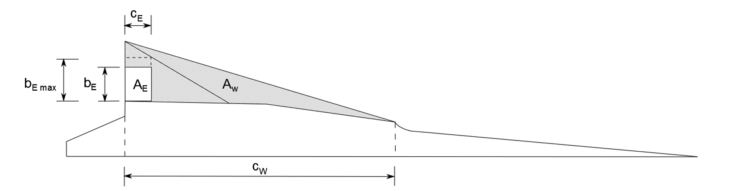
\includegraphics[width=0.8\linewidth]{figures/2_literature-review/SPARTANElevons}
 	\caption{The elevons of the SPARTAN\cite{Preller2017b}.}
 	\label{fig:SPARTANElevons}
 \end{figure}
 
  The scramjet accelerator stage of the SPARTAN was first designed by Jazra, Preller and Smart\cite{Jazra2010, Jazra2013}, based on the winged-cone vehicle developed by Shaughnessy et al. as part of the NASP program\cite{Shaughnessy1990}. 
  The scramjet accelerator has been sized to be 22.94m long, with an 8.90m wingspan, and is powered by four rectangular-to-elliptical shape transition (REST) scramjet engines, developed at The University of Queensland, specifically designed to integrate smoothly with the conical forebody of the scramjet accelerator. Elevons are included on the wings of the scramjet accelerator for primary control, shown in Figure \ref{fig:SPARTANElevons}. These elevons were sized through variation of the width, $b_E$, to have an area equal to 15\% of the area of the wing, and to have a cord length, $c_E$, of 15\% of the cord length of the wing\cite{Preller2018a}.
  Three retractable landing gear assemblies are included on the scramjet accelerator, shown in Figure \ref{fig:SPARTAN-Dawid}, so that the scramjet stage may be returned and landed in the same manner as a traditional aircraft; horizontally on a specially purposed runway. 
  
  \begin{figure}[ht]
  	\centering
  	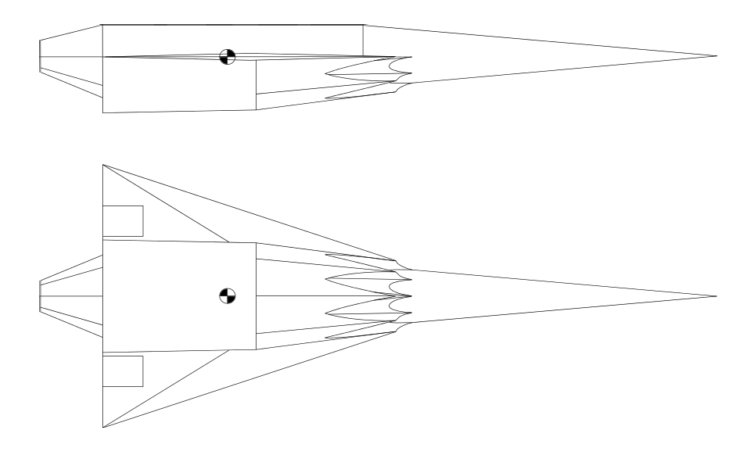
\includegraphics[width=0.9\linewidth]{figures/2_literature-review/SPARTAN-Dawid}
  	\caption{The scramjet accelerator of the SPARTAN, as designed by Preller\cite{Preller2018a}.}
  	\label{fig:SPARTAN-Dawid}
  \end{figure}
  
   \begin{figure}[!ht]
   	\centering
   	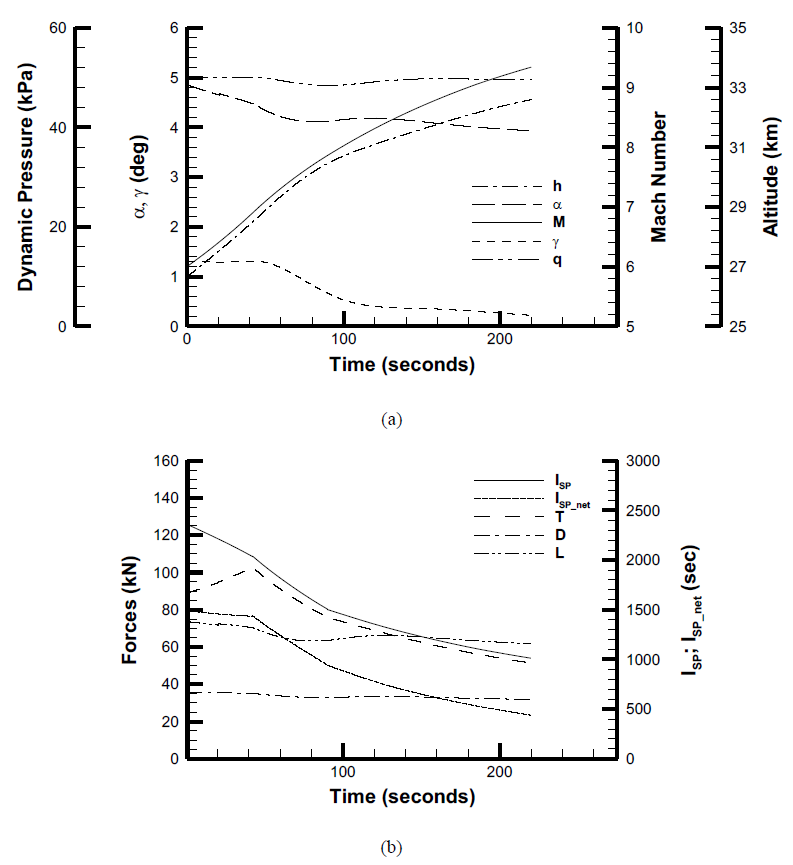
\includegraphics[width=0.9\linewidth]{figures/2_literature-review/SPARTAN_traj1}
   	\caption{The flight trajectory of the SPARTAN. a) shows the physical trajectory and b) shows the forces on the vehicle and performance indicators.}
   	\label{fig:SPARTAN_traj}
   \end{figure}
  
   To date, studies of the SPARTAN have assumed that the most efficient launch trajectory is achieved when the scramjet accelerator stage is constrained to fly at a constant dynamic pressure\cite{Preller2017b,Preller2018a}.
  Figure \ref{fig:SPARTAN_traj} shows the trajectory of the scramjet accelerator, simulated in three degrees of freedom to fly close to a constant 50kPa dynamic pressure, using a pole-placement angle of attack controller\cite{Preller2017b}.
  The ascent trajectory of the SPARTAN begins at Mach 6, and terminates at Mach 9.34, when the hydrogen fuel is exhausted\cite{Preller2018a}. 
  The net specific impulse of the SPARTAN varies from 1492s at the beginning of the trajectory, to 439s by the time the fuel is depleted\cite{Preller2017b}. 
  The SPARTAN is trimmed throughout the trajectory by ailerons on the wing, shown in Figure \ref{fig:SPARTANElevons}. Over the flight of the SPARTAN, the flap deflection changes from 10.6$^\circ$ to 12.2$^\circ$\cite{Preller2018a}. The drag contribution of the flap varies from 14.3\% to 14.5\%, and the lift contribution from 18.8\% to 21.0\%\cite{Preller2018a}. However, this is calculated without a detailed analysis of the centre of gravity location, which is assumed to be located at 50\% planform area. 
  Past studies of the scramjet accelerator vehicle have assumed that a fly-back to launch site is possible after third stage separation\cite{Preller2017b,Preller2018a}. However, this fly-back has not yet been simulated. 
  
 

The first stage rocket of the SPARTAN is launched vertically, accelerating the scramjet accelerator to its minimum operable Mach number. The first stage has not yet been modelled in detail, with only very representative aerodynamic models used for an analysis of a representative first stage rocket.
It is eventually intended that the first stage of the SPARTAN be returnable to launch site under cruise-back power for reuse, however, a first stage capable of return flight has not been designed or modelled for a full scale SPARTAN system\cite{Preller2017b,Preller2018a}.
 Some preliminary work has been carried out, exploring the reuse of the first stage boosters of the SPARTAN \cite{chai2017} for a modified, reduced size SPARTAN concept, however this work is still in its infancy, and the basic design of the booster or boosters is still to be determined\cite{Preller2017b,Preller2018a}.
 
  

The third stage of the SPARTAN is an expendable rocket system, that consists of a rocket motor, fuel tanks, structure, payload and a thermal protection system\cite{Preller2017b}, shown in Figure \ref{fig:ThirdStage}. The third stage has to this point been designed to be powered by the Pratt \& Whitney RL-10-3A\cite{Preller2017b}, and has exhibited good performance when powered by this engine. However, the RL-10-3A is a pump-fed engine, and is likely to be prohibitively expensive for a small launch system.
\begin{figure}[ht]
	\centering
	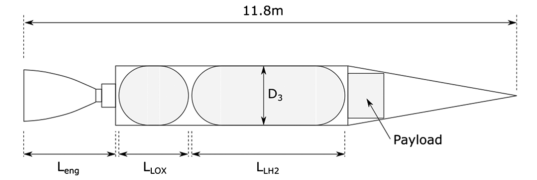
\includegraphics[width=0.7\linewidth]{figures/2_literature-review/ThirdStage}
	\caption{The third stage rocket of the rocket-scramjet-rocket launch system\cite{Preller2017b}.}
	\label{fig:ThirdStage}
\end{figure}
 Initially, the third stage was designed to be situated within the fuselage of the SPARTAN's scramjet accelerator, in the nose cone\cite{Jazra2013}. This design was changed by Preller\cite{Preller2018a,Preller2017b}, so that the rocket was situated in 'piggyback' position at the top of the fuselage as shown in Figure \ref{fig:SPARTAN-Dawid}. Rather than being situated entirely within the fuselage, the third stage was designed to fit into a recess into the back of the vehicle, to aid in high dynamic pressure separation. However, the effect of this recess on the aerodynamics of the scramjet accelerator after separation has not been considered\cite{Preller2018a,Preller2017b}. It is likely that this recess would have a large effect on the aerodynamics and controllability of the vehicle, particularly at high Mach numbers, where large areas of separation and recirculation are likely to be present. 





 
 \begin{figure}[ht]
 	\centering
 	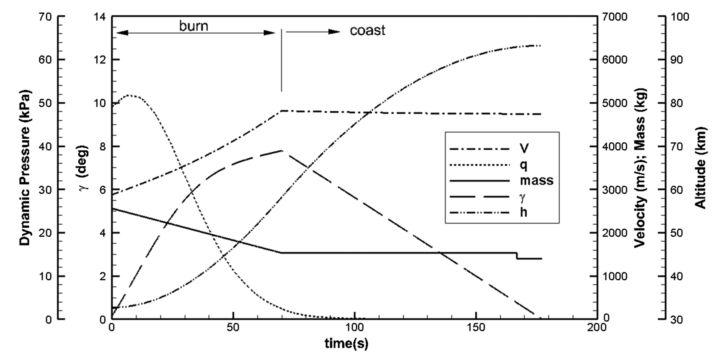
\includegraphics[width=0.9\linewidth]{figures/2_literature-review/SPARTAN_trajthirdstage}
 	\caption{The third stage trajectory of the SPARTAN launch system\cite{Preller2018a}.}
 	\label{fig:SPARTAN_trajthirdstage}
 \end{figure}

The trajectory of the third stage has to date been constrained to the scramjet accelerator flying a constant dynamic pressure trajectory, releasing the third stage into a high dynamic pressure environment. This trajectory, shown in Figure \ref{fig:SPARTAN_trajthirdstage}, uses a constant 10$^\circ$ angle of attack throughout, enabling the third stage to pull-up out of the atmosphere.  
 Once the density of the atmosphere is low enough, the thermal protection system separated from the vehicle for mass efficiency, and once exoatmospheric, the third stage performs a Hohmann transfer to reach the desired orbit. 
This trajectory enables the delivery of 279.8kg\cite{Preller2018a} of payload to sun synchronous orbit when using a third stage powered by a Pratt \& Whitney RL-10-3A\cite{Preller2018a}. 

Whilst the SPARTAN launch system is the most studied 3STO airbreathing system, it is evident that there is significant portions of the system left to design in detail, and significant design challenges to overcome. It is also apparent that the trajectory analysis of the SPARTAN, like all 3STO launch systems, and many 2STO launch systems, makes significant assumptions as to the most optimal flight path, notably constraining the scramjet accelerator to constant dynamic pressure flight. 
As previous studies have indicated\cite{Preller2017b}, if the performance and designs of this launch system and 3STO airbreathing launch systems in general are to be improved, the development and analysis of an optimal launch trajectory is necessary.



%\textcolor{red}{numbers are from prellers thesis, not paper.}



\section{Optimal Control}\label{sec:Optimisation}





\textcolor{red}{To investigate the best possible way of flying a rocket-scramjet-rocket launch system to orbit, a simulation must be developed that will calculate the optimal flight path, taking into account the trajectory of all of three stages of the launch system, including ascent trajectories, as well as the return to base of the scramjet accelerator stage. Calculating an optimal trajectory that combines all phases of a partially reusable, partially airbreathing, three-stage launch system is a complex task, that has not been carried out to-date.
Defining the trajectory of a launch system with multiple stages and multiple modes of propulsion purely from an a priori vehicle analysis is unlikely to yield a trajectory that maximises the performance of the system, due to the highly nonlinear performance of a multi-stage, multi-propulsion mode launch system, and the complex trade-offs that are present between the stages. The effects of these trade-offs are extremely difficult to predict, particularly because of the high sensitivity of airbreathing engines to flight conditions, and the complex aerodynamics of an airbreathing launch system. 
A method of determining the optimal flight path is required, that is able to maximise the performance of the launch system with very few assumptions as to the shape of the trajectory. 
}

\textcolor{red}{
Optimal control theory is used in situations where a control sequence must be found to produce an optimal trajectory with little prior knowledge of the form that the optimal trajectory will take. 
Optimal control theory is a general term for the mathematics of optimising a time variant dynamic system, that can be controlled. 
Optimal control theory is distinct from control theory in that it does not necessarily attempt to match a set reference or goal, as is generally the case for trajectories developed using control theory methods such as feedback control. Rather, a single global objective function is minimised by determining optimised control actions across the trajectory, subject to a set of user defined constraints.  
Optimal control theory has been widely used in aerospace applications, and has been successfully used to optimise the launch of airbreathing hypersonic launch vehicles\cite{Powell1991,Lu1993,Trefny1999,Roche2000,Pescetelli2012,Young2006}, including some of the trajectories detailed in Section \ref{sec:AscentTrajectories}. 
}

For an optimisation of a complex trajectory there are a variety of optimal control methods that are useful for specific problem types. These are separated into two categories: direct and indirect solution methods\cite{Betts1998}. Indirect methods are based on the calculus of variations or minimum principle model, and generally result in high accuracy solutions to optimisation problems\cite{Bulirsch1993}. However indirect models suffer from the drawbacks of small radii of convergence and the fact that the equations to be solved often exhibit strong nonlinearity and discontinuities. This means that indirect methods will not be solvable unless the problem is very well defined with a minimum of nonlinearity, making indirect methods unsuitable for many complex optimisation problems, such as aerospace vehicle simulations which can exhibit strong nonlinear behaviour and have a wide solution space. 

Direct methods transform an optimisation problem into a nonlinear programming (NLP) problem which can be solved computationally\cite{Stryk1992}. NLP solvers solve the optimisation problem defined as\cite{Bazaraa2013}:

\begin{equation}
Minimise \qquad f(x)
\end{equation}

\begin{equation}
Subject \quad to \qquad g_i(x)\leq0 \quad for \quad i=1,...,m
\end{equation}

\begin{equation}
and \qquad h_j(x) = 0 \quad for \quad j=1,...,n
\end{equation}

An optimisation problem that has been discretised in this form can thus be solved using any of a variety of NLP solvers. One of the most effective methods of solving twice differentiable NLP problems is sequential quadratic programming (SQP)\cite{Boggs2000} for which there is a variety of commercial solvers available such as NPSOL, SNOPT, and packages within MATLAB. 

In order for these packages to be able to solve an optimisation problem it must be presented in discretised form, and as such must be transformed using transcription techniques\cite{Kelly2015}. The task of transcribing a continuous optimisation problem into discrete NLP solvable form is not simple. SQP solvers can very easily run into convergence issues when provided with an optimisation problem which has not been well defined. Also, any transcription must be carried out with care that the accuracy of the solution is not compromised. 
There are multiple ways to approximate a continuous optimisation problem directly as an NLP problem, the most common of which are shooting and collocation methods. The choice of discretisation method can affect the stability and accuracy of the solution as well as the solution time of the problem. 

\subsection{Shooting Methods}

Shooting methods in optimal control are forward-time methods of discretisation\cite{Kelly2015}. Shooting methods explicitly enforce the dynamics of the system, and update the free conditions and system controls to move towards an optimal solution from an initial guess\cite{Kelly2015}. Shooting methods are generally simple to apply, and require little specialised knowledge to use once they have been implemented. 


\subsubsection{The Single Shooting Method}

The oldest and simplest method of approximating continuous optimisation problems as NLP problems is the direct single shooting method. Direct single shooting discretises the control function over the solution space, and solves this directly as an NLP by integrating the vehicle dynamics, or state variables, along the trajectory at each trajectory guess\cite{Betts1998,Kelly2015,Rao2009,Fasano2013}. \textcolor{red}{Figure \ref{fig:multipleshooting} illustrates the single shooting method, with green points indicating the start and end points, and red dots indicating the discretisation of the trajectory path. The vehicle dynamics are solved over these discretised time points directly, with controls modified to minimise an end target.} Single shooting is simple to apply and has been used since the 1970s for rocket trajectory optimisation\cite{jezewski1971}. \textcolor{red}{Single shooting methods have also been used for the analysis of airbreathing launch trajectories, with some degree of success\cite{Powell1991,Bradford2000,Hyperion,Bradford2002,Fujikawa2017}. However,} single shooting methods suffer from nonlinearity problems, ie. an optimisation problem solved using the single shooting method will potentially struggle to solve if the problem exhibits even small nonlinearities, due to being unable to converge to an optimal solution. This makes the single shooting method unsuitable \textcolor{red}{for the in-depth trajectory analysis of} complex problems such as a scramjet model, as there are many nonlinear factors inherent in atmosphere and airbreathing engine modelling. \textcolor{red}{For this reason single shooting is not commonly used at the current time for the trajectory analysis of complex launch vehicles.}


\subsubsection{The Multiple Shooting Method}

Direct multiple shooting solves some of the instabilities of the single shooting method by splitting the trajectory into multiple shooting arcs, and collocating these at specific time points\cite{Betts1998,Kelly2015,Rao2009,Fasano2013}. This creates a system of discontinuities, illustrated in Figure \ref{fig:multipleshooting}, which are gradually minimised by the solver algorithm until the trajectory is continuous. These discontinuities allow greater flexibility for the solver than is afforded by the single shooting method. 

\begin{figure}[ht]
	\centering
	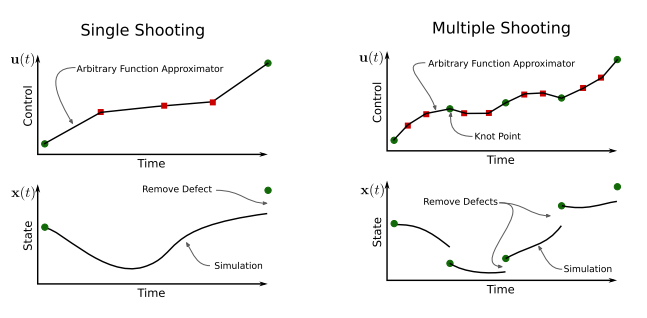
\includegraphics[width=0.9\linewidth]{SingleMultiple}
	\caption{A comparison of single shooting and multiple shooting\cite{Kelly2015}.}
	\label{fig:multipleshooting}
\end{figure}

The multiple shooting method has greatly improved convergence compared to the single shooting method, removing much of the susceptibility to instabilities resulting from nonlinear effects. For this reason, multiple shooting has been used successfully in a variety of applications, including the trajectory optimisation of reusable space vehicles\cite{Maddock2018}. However, the multiple shooting approach still suffers from a relatively small radius of convergence and slow computation times\cite{Fasano2013}. Radius of convergence is extremely important to this study as the optimal solution cannot be approximated to a great degree of accuracy. As such it is desirable to use a method with a large radius of convergence to apply to the optimisation problem being considered, to improve the robustness of the solution process.

\subsection{Collocation Methods}

Collocation methods are arguably the most powerful methods for solving optimal control problems\cite{Rao2009}. Collocation methods are simultaneous methods, where both the states and controls are approximated using a specific form of functional\cite{Kelly2015,Rao2009}. In these methods, the dynamics of the system are not explicitly enforced, but instead are constrained at specified points along the trajectory, called collocation points, or nodes\cite{Kelly2015}\textcolor{red}{, with the trajectory often divided into multiple segments at specific nodes, called 'knot' points. These nodes and knot points are illustrated for a pseudospectral method of collocation in Figure \ref{fig:HPExamples}, showing the relationship between the segments and nodes used, and the orthogonal polynomials that approximate the states and controls of the system being optimised. Constraining the dynamics in this way means} that the derivative of the state functions become a constraint within the NLP, being equated to the polynomial approximation functions by the solver algorithm. 
Collocation methods provide larger radius of convergence, greater robustness, and smaller computational times compared to multiple shooting\cite{Fasano2013}. However, the solution accuracy of collocation methods is less than that of multiple shooting methods\cite{Fasano2013}, although this can be improved through the choice of basis functions used for collocation\cite{Rao2009}.

Collocation methods can be represented in two ways; \textsf{h} and \textsf{p} schemes\cite{Kelly2015}. \textsf{p} schemes, or global methods, represent the entire trajectory as high order polynomials, and converge by increasing the order of these polynomial\cite{Kelly2015}. This method works well if the underlying solution is smooth, however, if there are discontinuities present, a \textsf{p} scheme will fail\cite{Kelly2015}. \textsf{h} schemes separate the trajectory into a series of medium order polynomials, stitched together at knot points using defect constraints, similarly to the multiple shooting method\cite{Kelly2015,Rao2009,Ross2004}. These joining points are called knot points\cite{Kelly2015,Ross2004}. A comparison between \textsf{h} and \textsf{p} methods is shown in Figure \ref{fig:HPExamples}.

\begin{figure}[ht]
	\centering
	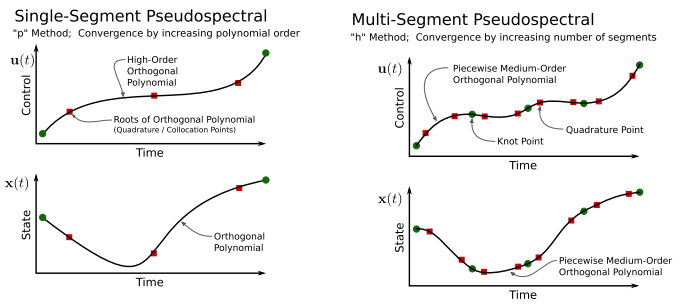
\includegraphics[width=0.9\linewidth]{figures/2_literature-review/HPExamples}
	\caption{Examples of \textsf{h} and \textsf{p} collocation methods\cite{Kelly2015}.}
	\label{fig:HPExamples}
\end{figure}

\subsubsection{The Pseudospectral Method}\label{sec:PS}


The most accurate and effective type of collocation methods use orthogonal polynomials to approximate the state and control functionals\cite{Fahroo2000}. In trajectory optimisation, this type of collocation is referred to as the pseudospectral method\cite{Kelly2015}. 
The pseudospectral method was first introduced in 1972 by Kreiss \& Oliger\cite{Kreiss1972} as an efficient way to compute meteorology and oceanography problems. The pseudospectral method has recently garnered a large amount of attention for its ability to rapidly and accurately solve a wide variety of optimal control problems.  When a solution is well behaved and smooth, the pseudospectral method converges at an exponential rate, with a high accuracy known as spectral accuracy\cite{Ross2004,Darby2011a}. 

The pseudospectral method employs the use of orthogonal polynomials such as Legendre or Chebychev polynomials to approximate the state and control functions.
This approximation is used to transcribe the optimal control problem into a nonlinear programming problem (NLP) through collocation. This process involves mapping the time domain of the system is to the time interval $[-1,+1]$, and discretising the approximated dynamics at a specific set of points, obtained from Gaussian quadrature\cite{Fahroo2000,Huntington2007,Kelly2015,Rao2009,Garg2011}. 
There are multiple types of pseudpospectral methods, distinguished by the polynomial and collocation points used. Usually, these polynomials are Chebyshev or Lagrange polynomials\cite{Fahroo2000,Rao2009}, and the collocation points are the roots of a Legendre polynomial\cite{Garg2009}. Chebyshev polynomials have been used since the introduction of pseudospectral methods in optimal control, but have been superseded in many cases by Lagrange polynomials, which offer simpler collocation conditions\cite{Rao2009}. 
There are many possible types of collocation nodes, although there are three most commonly used sets; Legendre-Gauss (LG); Legendre-Gauss-Radau (LGR); and Legendre-Gauss-Lobatto (LGL)\cite{Garg2009,Rao2009}. The choice of collocation type determines how the roots of the problem are calculated, and changes the formulation of the problem slightly\cite{Garg2009}. Practically, there is very little difference between these node sets\cite{Garg2009}.
Detailed information on the pseudospectral information may be found in Reference \cite{Huntington2007}.


The pseudospectral method is usually employed as a \textsf{p} method, where a global polynomial is used, and convergence is achieved by increasing the order of this polynomial\cite{Rao2009}. Recently, \textsf{hp}-adaptive pseudospectral methods have been introduced, which segment the mesh using an h method, whilst also having a variable polynomial degree, as in the \textsf{p} method\cite{Darby2011a}. These \textsf{hp} methods converge by varying the degree of the approximating polynomial as well as the number of segments simultaneously. Utilising both \textsf{h} and \textsf{p} methods improves the accuracy and robustness of the solution, as illustrated in Figure \ref{fig:OptimisationMethodComparisonChai}, from a study by Chai et al.\cite{Chai2015} comparing the single shooting method to non-adaptive and \textsf{hp}-adaptive pseudospectral methods. \textcolor{red}{This figure illustrates a comparison of a boost-skip hypersonic vehicle optimised for maximum range. All trajectories are relatively similar, however the \textsf{hp}-adaptive method is able to achieve slightly more range by redistributing nodes effectively. The \textsf{hp}-adaptive method also exhibits higher solution accuracy; in this problem the scramjet is limited to ignite at less than 1500m/s, and the \textsf{hp}-adaptive method ignites the scramjet at exactly 1500m/s, while the non-adaptive method ignited at 1499.256m/s, and the direct shooting at 1499.548m/s. This is a slight difference, but illustrates the improved capability of the \textsf{hp}-adaptive method to converge to specific optimal points. In addition to improved robustness and accuracy, the \textsf{hp}-adaptive method exhibits greater computational efficiency than the other methods, taking 5.3s in total to run this optimisation, compared to 12.7s for a non-adaptive method, and 268.2s for the direct shooting approach. In general the \textsf{hp}-adaptive method decreases the computational effort and memory usage necessary during the solution process by converging more rapidly to an optimal result\cite{Darby2011a,Chai2015}. }


\begin{figure}[ht]
	\centering
	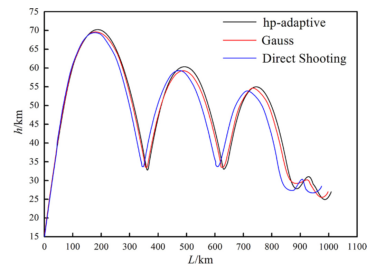
\includegraphics[width=0.7\linewidth]{figures/2_literature-review/OptimisationMethodComparisonChai}
	\caption{Comparison of optimisation techniques\cite{Chai2015}. A hypersonic vehicle is optimised for maximum range. The \textsf{hp}-adaptive method can be observed to have produced the most optimal result.}
	\label{fig:OptimisationMethodComparisonChai}
\end{figure}

A secondary usability advantage of the pseudospectral method is the ability to generate Hamiltonian and costate values easily\cite{Gong2010,Fahroo2001,Rao2009}. The Hamiltonian and costate values allow a solution to easily and quickly be checked to determine if some of the necessary conditions for optimality are being met. This is useful to determine if the optimal solution calculated by the pseudospectral solver is valid.


The pseudospectral method has been proven to be extremely effective for simulations in aerospace applications and has been proven in flight applications such as the zero propellant manoeuvre of the International Space Station in 2007, where the ISS was rotated 180 degrees without any propellant used following a pseudospectral method solution\cite{Bedrossian}. 
\textcolor{red}{
The pseudospectral method has been used successfully in a multitude of studies for the trajectory analysis of hypersonic vehicles\cite{Li2012,Josselyn2002a,Zhao2013,Tian2011,Darby2011,Chai2015,Rizvi2015,Moshman2014,Yang2017,Kodera2014}, and has proved an extremely effective tool for solving the highly nonlinear trajectory optimisation problems that arise from complex aerodynamics. 
These successful use cases indicate that the pseudospectral method is robust for complex, nonlinear systems, and that the pseudospectral method can be used to solver problems with many state variables and phases, such as is required by the aerodynamics and multi-stage nature of launch vehicles.
}
\section{Available Optimal Control Solvers}\label{sec:optsolvers}

There are a number of optimal control solvers available, both commercially and open source, that represent well tested implementations of state of the art pseudospectral methods. A summary of the most prominent available solvers is shown in Table \ref{table:programs}. These programs are mostly general solvers, and must be configured specifically in order to solve a particular optimal control problem. The exception is ASTOS\cite{astos}, which is a standalone program designed for aerospace trajectory optimisation.

Functionally, most of the available solvers are similar in operation. The states and controls of the optimal control problem are defined to the program by the user, along with any constraints; continuous or endpoint. The cost function of the problem is input, and dynamic model of the system is defined. An initial guess is provided, and once activated, the solver will move toward an optimal solution from this initial guess. 
The most significant practical difference between the solvers lies in the robustness of the optimal solution, ie. how easily a particular solver is able to converge to the optimal solution. For a simple and continuous optimisation problem all solvers will be able to approach the same solution (though with varying efficiency). However, for a complex and nonlinear optimisation problem, some solvers will converge much more easily and rapidly than others. Generally, this stems from the underlying transcription method used. 
The most common form of discretisation used by these solvers is the pseudospectral method, although other forms of collocation, as well as multiple shooting, are also used. Of the methods used, \textsf{hp}-adaptive pseudospectral methods exhibit the best convergence and accuracy properties\cite{Chai2015}. The readily available packages which utilise \textsf{hp}-adaptive pseudospectral methods are GPOPS-2\cite{Rao2010} and ICLOCS2\cite{iclocs}. Both ICLOCS2 and GPOPS-2 uses IPOPT\cite{Wachter2006}, a widely used open source nonlinear optimisation package which utilises an interior point line search filter method. 

ICLOCS2 is a software package in the alpha stages of development, which is based upon ICLOCS, a multiple shooting solver\cite{iclocs}. ICLOCS2 is able to implement a range of transcription methods, including a \textsf{hp}-adaptive Legendre-Gauss Pseudospectral method\cite{iclocs}. As ICLOCS2 is relatively new at the time of writing, it has not yet been implemented in any published works and documentation is limited. 

GPOPS-2 is a proprietary \textsf{hp}-adaptive pseudospectral method solver, which implements a variety of \textsf{hp}-adaptive pseudospectral methods, so that the best method may be chosen for a given problem\cite{Rao2010}. GPOPS-2 is specifically designed to be as flexible as possible, to accommodate for a wide range of problem formulations\cite{Rao2010}. GPOPS-2 is well proven in aerospace applications, and has been used for spacecraft orbit optimisation as well as in-atmosphere trajectory optimisation\cite{Rizvi2015,Lipp2014}. GPOPS-2 is well suited to solving multi-phase optimal control problems, which is necessary for efficient multi-stage launch optimisation\cite{Rao2010}. GPOPS-2 represents the state of the art in trajectory optimisation software, and as such is used by a number of institutions around the world. 



\begin{table}[ht]
	
	\begin{tabular}{|c|c|c| p{4cm}|}
		\hline \textbf{Software} & \textbf{Publisher} & \textbf{Platform} & \textbf{Optimisation Type} \\ 
		\hline DIDO\cite{Ross2002} & Elissar Global & MATLAB & Chebychev Pseudospectral \\ 
		\hline GPOPS II\cite{Rao2010} & RP Optimization Research & MATLAB & \textsf{hp}-Adaptive Legendre-Gauss-Radau Pseudospectral \\ 
		\hline PROPT (IPOPT)\cite{Rutquist2010}& TOMLAB & MATLAB & Legendre-Gauss  Pseudospectral  \\ 
		\hline ICLOCS2\cite{iclocs} & Imperial College & MATLAB &  Multiple Shooting / \textsf{hp}-adaptive Legendre-Gauss Pseudospectral  \\ 
		\hline POST2\cite{WilliamColson} & NASA & FORTRAN & Direct Shooting \\ 
		\hline OTIS\cite{otis} & NASA  & Fortran & Pseudospectral + Various  \\ 
		\hline TRANSWORHP\cite{Wassel2013} & ESA & Fortran/C++ & Full Discretisation \\ 
		\hline ASTOS\cite{astos} & Astos Solutions & Standalone & Multiple Shooting/Collocation  \\  
		\hline ACADO\cite{Houska2011} & Open Source & C++ &  Direct \\  
		\hline JModelica\cite{jmodelica} & Modelon AB, Open Source & Modelica/Python &  Collocation/ Pseudospectral \\  
		
		\hline 
	\end{tabular} 
	
	\caption{Summary of programs capable of pseudospectral optimisation.}
	\label{table:programs}
\end{table}

Although many of these optimisation packages are relatively similar, and are appropriate for highly nonlinear hypersonic launch problems, GPOPS-2 is the most readily available package that utilises a very high robustness and accuracy transcription method. However, GPOPS-2 is only a generic solver, requiring significant configuration to solve a launch problem. \textcolor{red}{This configuration includes launch vehicle modelling, and design of the optimal control problem, so that a solution maybe achieved. These are no small tasks, as the configuration of an optimal control problem for a complex launch vehicle requires deep knowledge of both the vehicle design and performance, as well as the underlying optimal control processes\cite{XXX}. } 














 







\section{Aerodynamic Analysis}

Optimising the trajectory of a space access vehicle using optimal control methods requires the input of a dynamic model of the launch vehicle. 
This dynamic model requires the aerodynamics of each stage of the launch system to be characterised at every flight condition experienced during launch. \textcolor{red}{This is usually achieved either analytically for simple vehicle designs, or through the generation of large aerodynamic coefficient databases that cover the operable region of the vehicle. The generation of databases is generally necessary when it is desired to capture more complex and nonlinear aerodynamics that must be pre-computed for efficiency.}

There are a variety of tools available to calculate the aerodynamics of aerospace vehicles.
 These tools are primarily designed towards either accuracy or efficiency, as more accurate methods require more computational power, longer computational times and, usually, more man-hours to produce a solution. 
This trade off means a tool must be selected which best suits the requirements of a given problem. 
For a preliminary vehicle design, it is often desirable to select a tool which is as computationally efficient as possible, as the design of the vehicle is liable to change often. 
Whereas for more advanced stages of vehicle design, an accurate tool is desirable, to assess the design of the vehicle in detail. 

The lowest fidelity, and highest efficiency methods include packages that use empirical relations derived from databases of existing vehicles, such as Missile Datcom\cite{Rosema2011}, as well as panel method codes such as HYPAERO\cite{Preller2017b}, cbaero\cite{Kinney2004} and HOTSOSE\cite{hotsose}. Low fidelity methods offer rapid solutions, with highly variable accuracy. For simple, standard vehicle shapes, low fidelity methods may be relatively accurate, as low fidelity solutions are usually calibrated to higher fidelity simulations or experiments. However, for complex vehicle geometries, for example geometries involving engine flow-paths, the accuracy of low fidelity models diminishes\cite{Krause2011}. \textcolor{red}{Despite this, low-fidelity codes are usually taken as being appropriate for preliminary design analysis, and are used in the analysis of all of the multi-stage airbreathing launch vehicles studies in Sections \ref{sec:twostagelaunchers} \& \ref{sec:threestage} where aerodynamic analysis is presented\cite{Wilhite1991,Fujikawa2017,Mehta2001,Takahashi1997,Germain2001,Eklund2012,Bradford2002,Kimura1999,Preller2018a}.} 

Medium fidelity methods consist of inviscid Euler solvers such as Cart3D\cite{CART3D} and FUN3D\cite{fun3d}, which are able to provide reasonable accuracy, with medium run times, by neglecting viscous effects within the solution. These solvers are often used in the later stages of preliminary design, or when higher fidelity is necessary due to design features, but rapid solutions are still desired.  Neglecting the viscous effects in the fluid flow means that the solution obtained from an inviscid solver will only be an approximation of the real flow, and that the accuracy of the solution varies depending on the type of problem being solved. For problems such as lift on a thin airfoil, inviscid Euler methods may be quite accurate, however for a problem such as boundary growth on a flat plate these methods will not accurately model the solution\cite{NASAEuler}. A particular advantage that many inviscid Euler codes provide is automatic adjoint mesh adaptation, the ability for the mesh to be automatically and rapidly generated, and updated sequentially throughout the solution process, refining areas of complex geometry or flow. This enables multiple solutions to be easily computed, without the need to regenerate meshes manually. In the early stages of vehicle design, inviscid-flow Euler CFD solvers are used extensively across industry and academia\cite{Almosnino2016}, as they are often able to capture \textcolor{red}{the trends in the aerodynamics of a launch vehicle sufficiently well for preliminary design purposes, while having relatively short run times that make the generation of aerodynamic databases practicable.}
 However, inviscid solvers naturally do not capture the aerodynamic forces on a vehicle due to viscous effects. This deficiency can be corrected using an approximation of the viscous forces, to improve the accuracy of the solution generated by an inviscid solver, while retaining the computational advantages of inviscid CFD\cite{Ward2018}. 

High fidelity methods consist of Navier-Stokes CFD solvers such as Eilmer3/4\cite{Gollan2013b}, Fluent\cite{Ansys2014}, CFX\cite{CFX}, COMSOL\cite{comsol}, TAU\cite{Schwamborn2006}, and OpenFOAM\cite{openfoam}. These solvers will resolve the fluid flow and aerodynamic forces to a high level of accuracy, including viscous effects. However, the mesh for the problem must be generated prior to the calculation of the solution, which increases the working time significantly. Additionally, the computation times are much longer, and require more computational resources than lower fidelity methods. These factors make the generation of an aerodynamic database using high fidelity CFD an extremely time consuming process. As such, high fidelity CFD is suited for use on mature vehicle designs, or when accurate flow simulation is judged to be necessary to \textcolor{red}{capture the behaviour of all or part of a vehicle. This is generally applied when the behaviour of the flow is particularly complex, or when the accurate calculation of the flow properties is necessary to assess aerodynamics or engine performance.}



\textcolor{red}{
\subsubsection{Cart3D}\label{sec:Cart3d}
}
\textcolor{red}{XXX Recheck this section for consistence after appendices done}

Cart3D is an inviscid Euler solver CFD package, designed for use during preliminary vehicle design and analysis\cite{Almosnino2016}. Cart3D is computationally efficient and requires only a surface triangulation of the vehicle being analysed to initiate a simulation. Cart3D is utilised in this study due to its balance of efficiency and ease of use, along with its reasonable accuracy for hypersonic flow calculations\textcolor{red}{XXX Cite}. Cart3D features adjoint mesh adaptation, and uses cartesian `cut-cells' that intersect the surface, allowing complex geometries to be analysed automatically. The mesh automatically refines as the simulation progresses, adaptively reducing error. The absence of a requirement for a user generated mesh allows Cart3D to be easily applied to complex launch vehicle designs, as well as allowing for simple modification of control surface deflections and flight conditions. 
Cart3D has been used extensively for aerodynamic simulations in preliminary design, including analysis of the plumes of the Skylon spaceplane\cite{Mehta2016}, HIFiRE-5\cite{Kimmel2010}, and in low sonic boom shape optimisations\cite{Aftosmis2011}. 
\begin{figure}[ht]
\centering
\includegraphics[width=0.6\linewidth]{figures/2_literature-review/Skylon-Cart3D}
\caption{The Skylon spaceplane, simulated using Cart3D at Mach 12.189, $\alpha=7.512^\circ$\cite{Mehta2016}. Cell distribution produced by mesh adaptation is shown.}
\label{fig:Skylon-Cart3D}
\end{figure}
Cart3D has shown fair agreement when compared to experimental and high-fidelity CFD results\textcolor{red}{XXX CIte}, particularly in the hypersonic regime, where the largest errors have been shown to be in the axial forces reported, due to the lack of viscous effects\textcolor{red}{XXX CIte}. 
It has been shown that if these viscous effects are corrected for, the accuracy of Cart3D for axial forces can be improved\textcolor{red}{XXX CIte}, making Cart3D fairly accurate in the hypersonic regime. Cart3D is used in this study for aerodynamic calculations, and its comparative performance is analysed in detail in Appendix XXX, utilising previous studies that compare Cart3D with experimental data and high fidelity CFD computations. 




      \textcolor{red}{
      \section{Summary}
    }

This section provided a review of available literature pertaining to the design and trajectory optimisation of a rocket-scramjet-rocket launch system.    
       Previous works on the design of airbreathing launch systems were detailed, separated into single, two-stage, and three-stage systems, and the launch trajectories of these systems were assessed. For single-stage systems it was generally shown that flight at maximum dynamic pressure under airbreathing operation, followed by a pull-up before transition to rocket power until orbit was considered the optimal trajectory. For two-stage launchers, this same type of trajectory was shown in many cases. However, the determination of the trajectory proved more complex, and often the booster stage only left maximum dynamic pressure in order to deliver the upper-stage to low-density atmospheric conditions. Some studies of two-stage launchers also showed trajectories that flew at off-maximum dynamic pressure conditions for the majority of airbreathing engine operation, or did not leave maximum dynamic pressure at all. Only two three-stage systems were identified, both following a prescribed maximum dynamic pressure flight path for the entirety of airbreathing engine operation. It was determined that a general optimal flight profile could not be developed for a three-stage airbreathing launch system.
       Due to being the most mature three-stage airbreathing concept, the SPARTAN rocket-scramjet-rocket launch system being developed by The University of Queensland and Hypersonix was investigated in detail, along with the trajectory simulations performed to-date. It was found that although multiple design studies of the SPARTAN have been conducted, the launch trajectory of this system has not yet been investigated in full, and no optimal trajectories have been investigated. 
       To assist ascent and return trajectory coupling, the return and maximum range trajectories of prior hypersonic vehicles were investigated, and it was determined that the return of a vehicle separated at hypersonic speeds is likely not possible without the operation of on-board engines. However, it was identified that performing a `skipping' manoeuvre may assist in maximising the glide range. 
       To facilitate the development of optimal trajectories, the background of optimal control theory was outlined, and the specific optimal control techniques that are most applicable to trajectory optimisation were detailed, along with a survey of existing optimal control solvers and their use-cases. 
	For vehicle aerodynamic modelling, a survey into CFD solvers was conducted, and the specific details of Cart3D and its uses for high-speed aerodynamics modelling were examined. 
